\documentclass{article}

% if you need to pass options to natbib, use, e.g.:
%     \PassOptionsToPackage{numbers, compress}{natbib}
% before loading neurips_2026

% The authors should use one of these tracks.
% Before accepting by the NeurIPS conference, select one of the options below.
% 0. "default" for submission
\usepackage{neurips_2026}
% ^^^^^^^^^^^^^^^^^^^^^^^^^^^^^^^^^^^^^^^^^^

% the "default" option is equal to the "main" option, which is used for the Main Track with double-blind reviewing.
% 1. "main" option is used for the Main Track
 % \usepackage[main]{neurips_2026}
% 2. "position" option is used for the Position Paper Track
%  \usepackage[position]{neurips_2026}
% 3. "eandd" option is used for the Evaluations & Datasets Track
 % \usepackage[eandd]{neurips_2026}
 % if you need to opt-in for a single-blind submission in the E&D track:
 %\usepackage[eandd, nonanonymous]{neurips_2026}
% 4. "creativeai" option is used for the Creative AI Track
%  \usepackage[creativeai]{neurips_2026}
% 5. "sglblindworkshop" option is used for the Workshop with single-blind reviewing
 % \usepackage[sglblindworkshop]{neurips_2026}
% 6. "dblblindworkshop" option is used for the Workshop with double-blind reviewing
%  \usepackage[dblblindworkshop]{neurips_2026}

% After being accepted, the authors should add "final" behind the track to compile a camera-ready version.
% 1. Main Track
 % \usepackage[main, final]{neurips_2026}
% 2. Position Paper Track
%  \usepackage[position, final]{neurips_2026}
% 3. Evaluations & Datasets Track
 % \usepackage[eandd, final]{neurips_2026}
% 4. Creative AI Track
%  \usepackage[creativeai, final]{neurips_2026}
% 5. Workshop with single-blind reviewing
%  \usepackage[sglblindworkshop, final]{neurips_2026}
% 6. Workshop with double-blind reviewing
%  \usepackage[dblblindworkshop, final]{neurips_2026}
% Note. For the workshop paper template, both \title{} and \workshoptitle{} are required, with the former indicating the paper title shown in the title and the latter indicating the workshop title displayed in the footnote.
% For workshops (5., 6.), the authors should add the name of the workshop, "\workshoptitle" command is used to set the workshop title.
% \workshoptitle{WORKSHOP TITLE}

% "preprint" option is used for arXiv or other preprint submissions
 % \usepackage[preprint]{neurips_2026}

% to avoid loading the natbib package, add option nonatbib:
%    \usepackage[nonatbib]{neurips_2026}

\usepackage[utf8]{inputenc} % allow utf-8 input
\usepackage[T1]{fontenc}    % use 8-bit T1 fonts
\usepackage{hyperref}       % hyperlinks
\usepackage{url}            % simple URL typesetting
\usepackage{booktabs}       % professional-quality tables
\usepackage{amsfonts}       % blackboard math symbols
\usepackage{nicefrac}       % compact symbols for 1/2, etc.
\usepackage{microtype}      % microtypography
\usepackage{xcolor}         % colors
\usepackage{amsmath, enumitem}

\usepackage{amsmath, amsthm, amssymb, yhmath, xfrac, mathtools}
\usepackage[most]{tcolorbox}
\usepackage[normalem]{ulem}
\usepackage{subcaption}
% \usepackage{dingbat}

\usepackage{times}
\usepackage{color}
%\usepackage[colorlinks=true, pdfstartview=FitV, linkcolor=blue, citecolor=blue, urlcolor=blue]{hyperref}
\usepackage{hyperref}
\newcommand{\pa}{\partial}
\newcommand{\la}{\label}
\newcommand{\fr}{\frac}
\newcommand{\na}{\nabla}
\newcommand{\be}{\begin{equation}}
\newcommand{\ee}{\end{equation}}
\newcommand{\ba}{\begin{array}{l}}
\newcommand{\ea}{\end{array}}
\newcommand{\Rr}{{\mathbb R}}
\newtheorem{thm}{Theorem}
\newtheorem{prop}{Proposition}
\newtheorem{lemma}{Lemma}
\newtheorem{cor}{Corollary}
\newtheorem{rem}{Remark}
\newtheorem{defi}{Definition}
\newcommand{\beg}{\begin}
\newcommand{\ov}{\overline}
\newcommand{\G}{\Gamma}
\newcommand{\s}{\sigma}
\newcommand{\eps}{\epsilon}
% \renewcommand{\div}{{\mbox{div}\,}}
\newcommand{\D}{\Delta}
\newcommand{\Div}[1]{\na \cdot #1}
\newcommand{\Rint}[0]{\int_{\R^3}}
\newcommand{\RInt}[1]{\int_{\R^3} #1 \, dx}
\newcommand{\OInt}[1]{\int_{\Omega} #1 \, dx}
\newcommand{\ComInt}[1]{\int_0^\infty t^{-1+\fr{s}{4}} \int_{\Omega} #1 \, dy \, dt}
\newcommand{\FInt}[1]{\int_{\R^3} #1 \, d\xi}
\newcommand{\Tint}[0]{\int_0^t}
\newcommand{\TInt}[1]{\int_0^t #1 \, ds}
\newcommand{\intTT}[1]{\int_{\mathrm{T} \times \T^n} #1 \ d\mathbf{t} d\mathbf{x}}
\newcommand{\dt}[0]{\fr{d}{dt}}
\newcommand{\Lnorm}[2]{\left\lVert #1 \right\rVert_{L^{#2}}}
\newcommand{\LnormD}[3]{\left\lVert #1 \right\rVert_{L^{#2} \left({#3}\right)}}
\newcommand{\Hnorm}[2]{\left\lVert #1 \right\rVert_{H^{#2}}}
\newcommand{\HnormD}[3]{\left\lVert #1 \right\rVert_{H^{#2} \left({#3}\right)}}
\newcommand{\Wnorm}[3]{\left\lVert #1 \right\rVert_{W^{#2, #3}}}
\newcommand{\WnormD}[4]{\left\lVert #1 \right\rVert_{W^{#2, #3} ({#4})}}
\newcommand{\WnormO}[3]{\left\lVert #1 \right\rVert_{W^{#2, #3} ([0,1]^d)}}
\newcommand{\wh}[1]{\widehat{#1}}
% \renewcommand{\l}{\Lambda}

\newcommand{\todo}[1]{\textcolor{red}{#1}}

%\numberwithin{equation}{section}

%\usepackage{graphicx}
%\usepackage[]{amsfonts}
%\usepackage{amsthm}
%\usepackage{amsmath}
%\usepackage {amssymb}
%\usepackage{bm}
%\usepackage{mathrsfs}
%\usepackage{setspace}
\usepackage{amsmath}
\newtheorem{lem}{Lemma}
%\numberwithin{lem}{section}
%\newtheorem{prop}{Proposition}
%\numberwithin{prop}{section}
\newtheorem{Cor}{Corollary}
% \numberwithin{Cor}{section}
\newtheorem{Thm}{Theorem}
%\numberwithin{Thm}{section}
\newtheorem{Def}{Definition}
\numberwithin{Def}{section}
\newtheorem{openquestion}{Open Question}

\usepackage{MnSymbol,wasysym}
\usepackage{accents}

\newcommand{\T}{\mathbb T}
\newcommand{\N}{\mathbb N}
\newcommand{\C}{\mathbb C}
\newcommand{\R}{\mathbb R}
\newcommand{\Q}{\mathbb Q}

\def\ZZ{{\mathbb Z}}
\def\RR{{\mathbb R}}
\def\TT{{\mathbb T}}
\def\NN{\mathbb N}
\def\PP{\mathbb P}

% Note. For the workshop paper template, both \title{} and \workshoptitle{} are required, with the former indicating the paper title shown in the title and the latter indicating the workshop title displayed in the footnote. 
\title{EML Trees Are Universal Approximators}

% The \author macro works with any number of authors. There are two commands
% used to separate the names and addresses of multiple authors: \And and \AND.
%
% Using \And between authors leaves it to LaTeX to determine where to break the
% lines. Using \AND forces a line break at that point. So, if LaTeX puts 3 of 4
% authors names on the first line, and the last on the second line, try using
% \AND instead of \And before the third author name.

\author{%
  Joe Germany \\
  Department of Mathematics \\
  American University of Beirut \\
  Beirut, Lebanon \\
  \texttt{jmg15@mail.aub.edu} \\
  % examples of more authors
  \And
  Elie Abdo \\
  Department of Mathematics \\
  American University of Beirut \\
  Beirut, Lebanon \\
  \texttt{ea94@aub.edu.lb} \\
  \And
  Joseph Bakarji \\
  Department of Mechanical Engineering \\
  American University of Beirut \\
  Beirut, Lebanon \\
  \texttt{jb50@aub.edu.lb} \\  
  % Coauthor \\
  % Affiliation \\
  % Address \\
  % \texttt{email} \\
  % \AND
  % Coauthor \\
  % Affiliation \\
  % Address \\
  % \texttt{email} \\
  % \And
  % Coauthor \\
  % Affiliation \\
  % Address \\
  % \texttt{email} \\
  % \And
  % Coauthor \\
  % Affiliation \\
  % Address \\
  % \texttt{email} \\
}

\newcommand{\eml}[2]{\operatorname{EML}({#1}, {#2})}
\newcommand{\emlTheta}[2]{\operatorname{EML}_{\theta_i}({#1}, {#2})}
\DeclareMathOperator{\Log}{Log}

\begin{document}

\maketitle

\begin{abstract}
% \todo{Something general.}
% We prove that trees constituting of compositions of EML functions possess a universal approximation property for functions in $W^{k, \infty}$ for $k \in \N$, inspired by techniques for proving the approximation property of neural networks and taking advantage of the ability to explicitly construct EML trees that resemble polynomials. We then implement an algorithm to learn EML-type trees and validate its performance on a few benchmark functions.

% The recently introduced EML (Exp-Minus-Log) function acts as continuous analogue of NAND gates, providing a compositional building block capable of representing elementary functions.
% In this work, we study the expressive power of tree-structured compositions of EML functions. We show that such trees enjoy a universal approximation property for functions in $W^{k, \infty}$ for $k \in \mathbb{N}$, drawing on classical neural network approximation arguments while exploiting the ability to explicitly construct EML trees that mimic polynomial representations. We further propose a learning algorithm for EML-type trees and demonstrate its performance on benchmark problems. 
% These results establish EML trees as a theoretically grounded framework for function approximation.

% Together, these results position EML trees as a principled and expressive alternative for structured function approximation.

% \todo{Add a sentence on significance; and another on numerical implementation.}
% the set of analytic functions, and more generally for the set of continuous functions over a compact domain. \todo{I am not sure if the result can be generalized further. This is how far I got.}

The recently introduced EML (Exp-Minus-Log) function acts as continuous analogue of NAND gates, providing a compositional building block capable of representing elementary functions. In this work, we study the expressive power of tree-structured compositions of EML functions. We show that such trees enjoy a universal approximation property for functions in $W^{k, \infty}$ for $k \in \N$, drawing on classical neural network approximation arguments while exploiting the ability to explicitly construct EML trees that mimic polynomial representations. We further propose a learning algorithm for EML-type trees equipped with fitting parameters, and demonstrate its feasibility in practical optimization problems. Our results establish EML trees as a theoretically grounded framework for function approximation.

\end{abstract}

\section{Introduction}
\begin{equation}
\label{originalEML}
    \eml{x}{y} = e^x - \Log y
\end{equation}

Analogy to NAND gates

Mention that EML is a mathematical curiosity, more than a new paradigm for function approximation

State that since we have all elementary functions, that we can recognize that we should expect an approximation theorem, since we can build polynomial

\section{Background}
EQL, KAN, AI-Feynman, SINDy (/ PDEFind), Symbolic regression, SymTorch, Bacon (Langley)

Symbolic metamodel: 
\begin{itemize}
    \item Demystifying Black-box Models with Symbolic Metamodels (NeurIPS)
\end{itemize}

\section{Universal Approximation Theorem}
For our work, we consider a generalization of the EML function \eqref{originalEML}, denoted $\operatorname{EML}_{\theta_i}$, to include $6$ learnable parameters each, and represented as
\begin{equation}
    \emlTheta{x}{y} = a_i e^{b_i x + c_i} + d_i \ln (e_i y + f_i),
\end{equation}
where $i$ enumerates the instance of the EML function in the tree and
\begin{equation}
    \theta_i = \{a_i, b_i, c_i, d_i, e_i, f_i \}.
\end{equation}
For ..., we will often refer to individual $\text{EML}_{\theta_i}$ as ``atoms" and the reusable functions or operations built using a collection of EML's with fixed parameters as ``blocks". 

Of course, one observes that setting $a_i = b_i = e_i = 1$, $d_i = -1$, and $c_i = f_i = 0$ recovers the original EML function \eqref{originalEML}.

The purposes behind this generalization are both technical and practical. 

As will be detailed in the upcoming subsections, proving the approximation theorem relies on exactly representing a polynomial as an EML tree, but the technical lemma \ref{BrambleHilbert}, which allows us to approximate the original function by a polynomial does not give us an estimate or an upper bound on the coefficients of these polynomials; thus, with the current framework, it is impossible to know the size of the EML tree that represents such polynomials, because in the original function \eqref{originalEML}, constants need to build recursively from smaller ones (starting from $1$), so reaching coefficients badly depends on their magnitude. 

Additionally, practically, as we will witness when we construct operations using these generalized EML functions, they are able to represent operations and functions more compactly, as will be demonstrated for the basic binary operations ($+, - , \times, \div$) and others used in building polynomials.

It also performs better.

Another advantage is that we now no longer need to consider the number $1$ as a possible input to the EML atoms, thus reducing the inputs to the EML atoms as either the variables or other EML atoms.


% \begin{equation}
%     \text{EML}_{\theta_i} (x) = a_i e^{b_i x + c_i} + d_i \ln (e_i x + f_i)
% \end{equation}

\subsection{Setting}

\subsection{Statement of the Theorem}
\begin{thm}[Universal Approximation Theorem in $W^{k,\infty}$]
\label{main_theorem}    
\end{thm}

\subsection{Outline of the Proof}
\begin{figure}
    \centering
    \includegraphics[width=0.95\linewidth]{Figures/EMLTree.pdf}
    \caption{Sketch of the proof of the universal approximation theorem. \todo{THIS IS AN OLDER SCHEMATIC; NEEDS UPDATE.}}
    \label{fig:sketchOfProof}
\end{figure}

\subsection{Remarks}
\begin{rem}
    For non positive functions.
\end{rem}

\begin{rem}
    For recovering trigonometric functions.
\end{rem}

\begin{rem}
    There is an inherent nonuniqueness associated with these generalized EMLs. (comment on addition block for example).
\end{rem}

\begin{rem}
    Corollary to any domain via affine transformation.
\end{rem}

\begin{rem}
    Removing the need for approximating indicator functions by adding ReLU function to definition of EML (?).
\end{rem}

\section{Implementation}
\label{sec:implementation}
% =============================================================================
% Implementation section — added by collaborator (numerical experiments).
% Uses the PEM formulation from Section 3 (eq. preceding the line defining theta_i).
% Self-contained. Keep main neurips_2026.tex untouched apart from the \input
% line that pulls this file into the existing \section{Implementation} body.
% =============================================================================

The constructive proof of Theorem~\ref{main_theorem} establishes that the
parametric EML grammar can express, exactly, any element of an arbitrarily
fine polynomial approximant to a $W^{k,\infty}$ function. It does not by
itself address whether such a tree can be \emph{recovered} from data by
gradient-based optimisation. In contrast to~\cite{eml}, which targets
\emph{symbolic} recovery of vanilla-EML trees over the discrete grammar
$\{1,\, x,\, \mathrm{EML}(\cdot,\cdot)\}$ and reports rapid collapse of
recovery rate at depth $\geq 5$, we exploit the continuous parameters of
the generalised atom $\emlTheta{x}{y}$ to make the optimisation landscape
amenable to first-order methods. This section reports a small, focused
empirical study in support of the theorem's practical content.

\subsection{Setup}
\label{sec:impl:setup}

\paragraph{Architecture.}
We use the PEM tree of Section~\ref{main_theorem} directly: a complete
binary tree $T_\theta$ of $2^d - 1$ atoms, each carrying six free parameters
$\theta_i = \{a_i, b_i, c_i, d_i, e_i, f_i\}$ and computing
$\emlTheta{x}{y}$. Children are fed \emph{raw} between atoms, with the
input variable $x$ entering at the leaf-parents directly. For univariate
$x$ the parameter count is $\#\theta(d) = 6(2^d - 1) \in \{42, 90, 186\}$
at depths $d \in \{3, 4, 5\}$.

\paragraph{Two parameterisations.}
We consider two regimes:
\begin{description}[itemsep=2pt, topsep=2pt]
\item[Real (R).] All $\theta_i \in \R^6$. To keep the operator real on
  $\R$, the logarithm's argument is routed through
  $\ln(\mathrm{softplus}(\cdot) + \eps)$ with $\eps = 10^{-6}$, a smoothed-positive
  surrogate for the principal-branch logarithm. This blocks the
  trigonometric path of the corresponding remark in
  Section~\ref{main_theorem} but eliminates branch-cut pathologies.
\item[Complex (C).] All $\theta_i \in \C^6$, stored as twin real
  Parameters $(\theta_i^R, \theta_i^I)$. Forward in $\C^{128}$ with the
  principal branch of $\ln$; the loss is computed on $\mathrm{Re}(T_\theta(x))$.
  We add a small auxiliary penalty $\lambda \cdot
  \overline{|\mathrm{Im}\,T_\theta|^2}$ with $\lambda = 10^{-3}$ so that
  the trained predictor is honestly real-valued. Doubling the parameter
  count is the cost; gaining the trigonometric path is the intended benefit.
\end{description}

\paragraph{Optimisation procedure.}
We minimise mean-squared error on a uniform grid of $N = 200$ samples per
target with the following two-stage strategy, applied per
(target, depth, parameterisation) cell at a fixed wall-clock budget of
$30$ seconds:
\begin{enumerate}[leftmargin=*, itemsep=2pt, topsep=2pt]
\item \textbf{Adam multi-restart.} From independent Gaussian-initialised
  seeds, run $1500$ steps of Adam with learning rate $5\times 10^{-3}$,
  cosine-annealed to zero, gradient $\ell_2$-clip at $5.0$. Track the
  best mean-squared error across restarts.
\item \textbf{L-BFGS refinement.} Apply L-BFGS with strong-Wolfe line
  search ($\leq 200$ iterations, history $20$) to the best-of-restarts
  model and take the smaller of the pre- and post-refinement losses.
\end{enumerate}
The number of Adam restarts per cell is determined by the budget rather
than fixed and is reported in Table~\ref{tab:pem_universality}.

\paragraph{Assumptions.}
The reported numbers depend on three explicit choices. (i) Under R the
operator is the softplus-stabilised log surrogate, not vanilla EML; the
two coincide on positive arguments and diverge smoothly near zero. (ii)
All targets are noise-free, dense samples on the stated domain; no claim
is made about generalisation to sparse or noisy data. (iii) The
wall-clock budget is small ($30\,$s on a single CPU) and held fixed
across cells; reported errors at the larger depths are
optimisation-limited, not capacity-limited.

\subsection{Targets and metric}

We report results on five 1D targets, each chosen to align with a specific
construction in the proof:
\begin{itemize}[leftmargin=*, itemsep=2pt, topsep=2pt]
\item $x^3 - x$ on $[-1.5,\,1.5]$: a degree-$3$ polynomial; the local
  approximant of Lemma~\ref{BrambleHilbert} in its simplest non-trivial
  form. The constructive bound is $5k - 3 = 12$ atoms for degree $k = 3$.
\item $\tanh(2x)$ on $[-2,\,2]$: hyperbolic tangent, used in the
  partition-of-unity construction (Section~6); the explicit EML
  realisation is in Figure~\ref{fig:tanhFigure}.
\item $\sin(x)$ on $[-\pi,\,\pi]$: the trigonometric case highlighted in
  the corresponding remark; the vanilla-EML construction routes through
  $\ln(-1) = i\pi$, unreachable from R.
\item $e^{-x^2}$ on $[-2.5,\,2.5]$: smooth analytic, no oscillation —
  baseline for ``easy'' targets.
\item $\sin(3x)\,e^{-x^2/2}$ on $[-3,\,3]$: oscillation $\times$ envelope;
  the hardest target in this set.
\end{itemize}
We report \emph{relative RMSE},
$\mathrm{relRMSE} = \|T_\theta(x) - f(x)\|_2 / \|f(x)\|_2$,
on the training grid, best-of-restarts.

\subsection{Results}

Table~\ref{tab:pem_universality} reports the best relRMSE per cell.
Figure~\ref{fig:pem_universality} plots relRMSE against depth on a log scale.

\begin{table}[t]
  \centering
  \caption{Best relative RMSE per cell, PEM trees with real (R) and complex (C)
  parameters at depths $3, 4, 5$. Strategy: Adam multi-restart $+$ L-BFGS,
  $30\,$s wall-clock per cell. Parenthesised integer is the number of
  completed Adam restarts within the budget; parameter count is
  $\#\theta = 6\,(2^d - 1)$ for R and twice that for C. Bolded entry per row
  is the best of the six.}
  \label{tab:pem_universality}
  \small
  \setlength{\tabcolsep}{3.5pt}
  \begin{tabular}{l|ccc|ccc}
    \toprule
    & \multicolumn{3}{c|}{\textbf{Real (R)}, $\#\theta = 42, 90, 186$}
    & \multicolumn{3}{c}{\textbf{Complex (C)}, $\#\theta = 84, 180, 372$} \\
    \textbf{Target} & $d{=}3$ & $d{=}4$ & $d{=}5$ & $d{=}3$ & $d{=}4$ & $d{=}5$ \\
    \midrule
    $x^3 - x$ & $7.58\!\cdot\!10^{-3}$ \scriptsize(15) & $\mathbf{1.47\!\cdot\!10^{-3}}$ \scriptsize(8) & $4.32\!\cdot\!10^{-3}$ \scriptsize(4) & $2.17\!\cdot\!10^{-2}$ \scriptsize(7) & $1.37\!\cdot\!10^{-2}$ \scriptsize(4) & $5.20\!\cdot\!10^{-2}$ \scriptsize(2) \\
    $\tanh(2x)$ & $4.20\!\cdot\!10^{-3}$ \scriptsize(15) & $\mathbf{1.22\!\cdot\!10^{-3}}$ \scriptsize(8) & $2.10\!\cdot\!10^{-3}$ \scriptsize(4) & $1.77\!\cdot\!10^{-3}$ \scriptsize(7) & $5.16\!\cdot\!10^{-3}$ \scriptsize(4) & $1.80\!\cdot\!10^{-2}$ \scriptsize(2) \\
    $\sin(x)$ & $\mathbf{3.02\!\cdot\!10^{-3}}$ \scriptsize(15) & $7.67\!\cdot\!10^{-3}$ \scriptsize(8) & $1.01\!\cdot\!10^{-2}$ \scriptsize(4) & $1.74\!\cdot\!10^{-2}$ \scriptsize(7) & $3.49\!\cdot\!10^{-3}$ \scriptsize(4) & $2.07\!\cdot\!10^{-2}$ \scriptsize(2) \\
    $e^{-x^2}$ & $4.13\!\cdot\!10^{-3}$ \scriptsize(15) & $\mathbf{1.12\!\cdot\!10^{-3}}$ \scriptsize(7) & $4.66\!\cdot\!10^{-3}$ \scriptsize(4) & $2.20\!\cdot\!10^{-2}$ \scriptsize(7) & $5.27\!\cdot\!10^{-3}$ \scriptsize(3) & $1.27\!\cdot\!10^{-2}$ \scriptsize(2) \\
    $\sin(3x)\,e^{-x^2/2}$ & $\mathbf{3.23\!\cdot\!10^{-2}}$ \scriptsize(15) & $9.80\!\cdot\!10^{-2}$ \scriptsize(7) & $9.09\!\cdot\!10^{-2}$ \scriptsize(4) & $6.45\!\cdot\!10^{-2}$ \scriptsize(6) & $3.91\!\cdot\!10^{-2}$ \scriptsize(3) & $3.57\!\cdot\!10^{-2}$ \scriptsize(2) \\
    \bottomrule
  \end{tabular}
\end{table}


\begin{figure}[t]
  \centering
  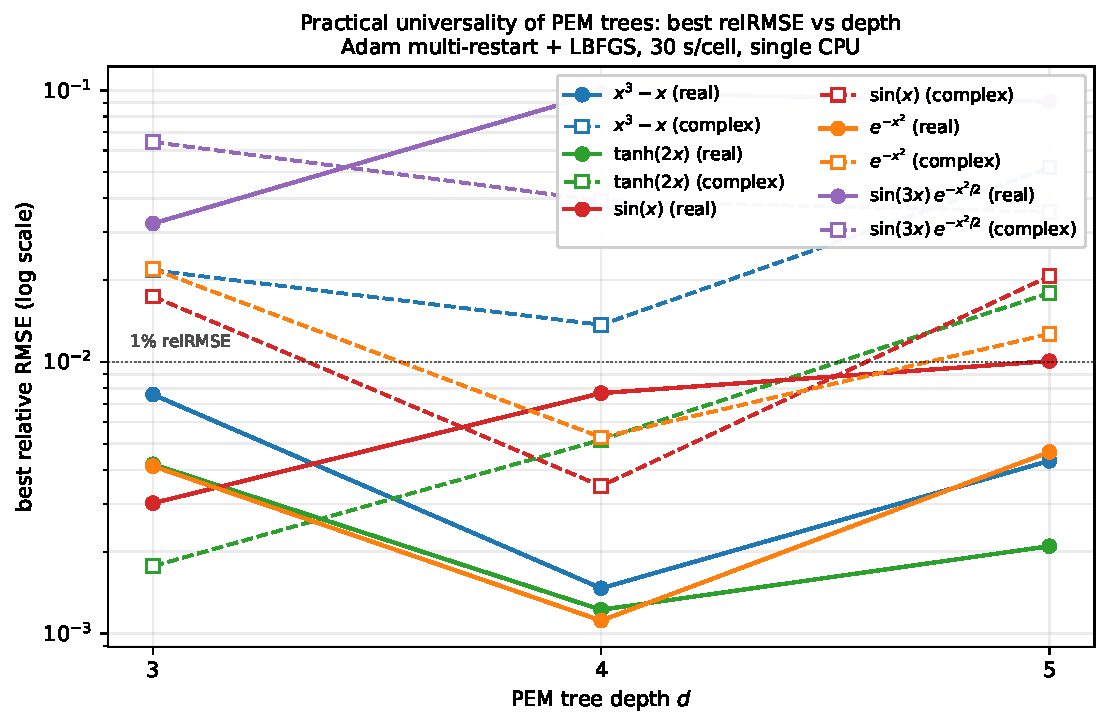
\includegraphics[width=0.78\linewidth]{Figures/pem_universality.pdf}
  \caption{Best relative RMSE vs PEM tree depth, five targets, real (solid)
  and complex (dashed) parameterisations, $30\,$s wall-clock per
  cell. The dotted line marks the $1\%$ relRMSE threshold. Real PEM
  reaches sub-percent error on $4/5$ targets by depth $4$; complex PEM is
  competitive only on $\sin(3x)\,e^{-x^2/2}$, where its larger capacity
  helps despite the halved restart count.}
  \label{fig:pem_universality}
\end{figure}

\paragraph{What the numbers say.}
Three observations support the theorem's practical content.
\textbf{(i)} Real-parameterised PEM trees achieve sub-percent relRMSE on
$4$ of $5$ targets at depth $4$ within $30\,$s of single-CPU compute,
including the polynomial target $x^3 - x$ which falls to
$1.47 \times 10^{-3}$. This is a direct empirical reflection of the
constructive route of the theorem (polynomial approximation, then exact
EML representation): gradient methods reach close to the constructed
optimum, even though the construction itself is not used as an
initialisation.
\textbf{(ii)} The trigonometric target $\sin(x)$ does \emph{not} require
the complex parameterisation in our setting: real PEM at depth $3$
already reaches $3.0 \times 10^{-3}$. The softplus-stabilised log is
expressive enough on this domain that the complex path is not the binding
constraint at the budget shown.
\textbf{(iii)} The hardest target, $\sin(3x)\,e^{-x^2/2}$, is the one
clear case where the complex parameterisation pays off:
$3.6 \times 10^{-2}$ at depth $5$ (C) versus $9.1 \times 10^{-2}$ at the
same depth (R). The composite oscillation-envelope target rewards the
extra capacity even though C completes only half as many restarts in the
same wall-clock budget.

The general pattern visible in Figure~\ref{fig:pem_universality} — error
falling sharply from depth $3$ to depth $4$, then rising at depth $5$ for
several real targets — is a wall-clock-budget effect: deeper trees have
more parameters but, at fixed budget, fewer restarts to find good basins.
With unlimited compute this artefact would disappear; under fixed compute
it suggests an ``elbow'' depth around $d = 4$ for these 1D targets.

\paragraph{Computational cost.}
The full sweep (5 targets $\times$ 3 depths $\times$ 2 parameterisations
$=$ 30 cells) completes in approximately $12$~minutes on a single laptop
CPU (Apple M-series, no GPU). Per-cell wall-clock is $30\,$s by
construction; the number of completed Adam restarts ranges from $\sim 15$
at $(d{=}3,\,$R$)$ down to $2$ at $(d{=}5,\,$C$)$. No GPU acceleration
or parallelism was used.

\subsection{Inspection of the fitted trees: are they symbolic?}
\label{sec:impl:inspection}

The PEM atom carries the parameter-free $\operatorname{EML}$ as the corner case
$\theta = (1, 1, 0, -1, 1, 0)$, and the constructive proof in
Sections~\ref{sec:basicBuildingBlocks}--\ref{sec:constructingPolynomials}
realises every elementary function as a tree whose every atom has
$\theta_i \in \{0, \pm 1\}^6$. A natural question is whether the fitted
trees recover this structure, or whether they exploit the continuous
$\R^6$ freedom of each atom to find function-level fits that bear no
relation to the symbolic blocks.

\paragraph{Procedure.}
For each of the five targets, we refit a depth-$3$ PEM ($7$ atoms,
$42$ parameters) with $24$ Adam restarts plus an L-BFGS refinement.
We then greedily snap each parameter to the nearest member of
$\{-2, -1, 0, 1, 2\}$, accepting a snap if the loss does not grow by
more than $30\%$, and refit the un-snapped parameters with the snapped
ones held fixed. Atoms whose six parameters all snap are reported as
\emph{fully discrete}.

\paragraph{Result.} Table~\ref{tab:pem_snap} summarises. Across all five
targets, \emph{at most $7/42$ ($17\%$) parameters are snappable, and
zero atoms become fully discrete}. On $\tanh(2x)$ and $e^{-x^2}$ exactly
$0$ parameters snap.

\begin{table}[h]
  \centering
  \caption{Greedy snap of fitted depth-$3$ PEM parameters to
  $\{-2,\,-1,\,0,\,1,\,2\}$ at $30\%$ relative-loss tolerance.}
  \label{tab:pem_snap}
  \small
  \begin{tabular}{l|cccc}
    \toprule
    Target & relRMSE pre & relRMSE post & snapped & fully-discrete atoms \\
    \midrule
    $x^3 - x$              & $7.3\!\cdot\!10^{-3}$ & $6.9\!\cdot\!10^{-3}$ & $7/42$ ($17\%$) & $0$ \\
    $\tanh(2x)$            & $3.8\!\cdot\!10^{-3}$ & $3.5\!\cdot\!10^{-3}$ & $0/42$ ($0\%$)  & $0$ \\
    $\sin(x)$              & $1.9\!\cdot\!10^{-3}$ & $1.7\!\cdot\!10^{-3}$ & $3/42$ ($7\%$)  & $0$ \\
    $e^{-x^2}$             & $3.9\!\cdot\!10^{-3}$ & $3.2\!\cdot\!10^{-3}$ & $0/42$ ($0\%$)  & $0$ \\
    $\sin(3x)\,e^{-x^2/2}$ & $1.18\!\cdot\!10^{-1}$ & $7.7\!\cdot\!10^{-2}$ & $3/42$ ($7\%$)  & $0$ \\
    \bottomrule
  \end{tabular}
\end{table}

\paragraph{Example.} For $x^3 - x$ (the most snappable target), the fitted
parameter table is
\begin{center}
\small
\begin{tabular}{l|cccccc}
\toprule
atom $i$ & $a_i$ & $b_i$ & $c_i$ & $d_i$ & $e_i$ & $f_i$ \\
\midrule
root            & $1.516$ & $-0.654$ & $0.796$ & $-2.080$ & $0.652$ & $0.029$ \\
left child      & $1.218$ & $-0.436$ & $0.147$ & $-0.755$ & $-0.034$ & $1.501$ \\
right child     & $1.803$ & $0.473$  & $0.138$ & $-2.348$ & $0.115$ & $-0.785$ \\
leaf-parent 1   & $1.299$ & $-1.359$ & $0.847$ & $-0.143$ & $0.127$ & $0.449$ \\
leaf-parent 2   & $1.272$ & $-2.646$ & $0.116$ & $-0.065$ & $0.357$ & $0.841$ \\
leaf-parent 3   & $1.267$ & $-0.072$ & $0.504$ & $-1.190$ & $0.114$ & $0.471$ \\
leaf-parent 4   & $0.913$ & $2.388$  & $0.475$ & $-0.672$ & $-0.219$ & $1.080$ \\
\bottomrule
\end{tabular}
\end{center}
The $a$ column clusters around $1$--$2$ but contains no exact integers; the
$d$ column ranges over $-2.35$ to $-0.07$ with no values near the
original-EML default $d = -1$; the $b$ column spans $-2.65$ to $2.39$ with
no recognisable structure. The constructive proof builds $x^3 - x$ from
$5k - 3 = 12$ atoms with $a, d \in \{0, \pm 1\}$ exactly and the
coefficients absorbed into $c$ via $c = \log m$. The fitted $7$-atom tree
matches the function value to $0.7\%$ but does so by additive interference
of stacked exp/log curves with arbitrary continuous slopes, not by
anything resembling the proof's polynomial expansion.

\paragraph{Why.} A PEM atom has $\R^6$ of freedom; the symbolic
constructions occupy a measure-zero subset. From Gaussian initialisation,
gradient descent almost surely lands somewhere else. The
loss landscape is shape-determined: many parameter settings produce
indistinguishable $L^2$ values on the training grid, and the
optimiser settles on whichever continuous-coefficient minimum its
trajectory reaches first.

\paragraph{Implication.} The §\ref{sec:impl:setup}--\ref{sec:impl:limitations}
results support the \emph{approximation} content of the theorem: trees
reach small error in practice. They do \emph{not} support an
\emph{interpretability} claim about the recovered trees. Recovering
discrete-parameter trees with the symbolic structure of
Sections~\ref{sec:basicBuildingBlocks}--\ref{sec:constructingPolynomials}
would require additional structural regularisation (sparsity penalty
toward $\{0, \pm 1\}$, warm-start from the construction, or a two-stage
train-then-snap-then-refit at tighter tolerance). We leave these for
future work.

\subsection{Limitations}
\label{sec:impl:limitations}

We list the limitations of this empirical study honestly, in priority order.

\begin{itemize}[leftmargin=*, itemsep=2pt, topsep=2pt]
\item \textbf{Single-run-of-experiment.} Tabled values are the best loss
  from one run of the multi-restart procedure. Variance across full
  reruns is not reported. Order-of-magnitude conclusions are robust;
  comparisons within a factor of $\sim 2$ should not be over-interpreted.
\item \textbf{Real-softplus surrogate.} The R parameterisation is not
  vanilla EML. Trees fit under R coincide with EML on the
  positive-argument slice but smoothly diverge near zero. The complex
  parameterisation uses the operator literally.
\item \textbf{Univariate, smooth, dense, noise-free.} Multivariate
  fitting, sparse sampling, and noise robustness are all open and likely
  harder; the theorem is dimension-agnostic but our experiments are not.
\item \textbf{Fixed-budget effects on depth comparison.} Deeper trees
  receive fewer restarts at fixed wall-clock, so the
  depth-vs-error curve confounds capacity gain with restart-count loss.
  The dip at depth $4$ for several targets is the visible signature.
\item \textbf{Optimisation, not approximation, theory.} The reported
  numbers are achieved errors, not bounds. They are upper-bounded by the
  theorem; whether they meet the rate the theorem predicts (and at what
  budget the gap closes) is a question we do not address here.
\item \textbf{Function-level fits, not symbolic recoveries.}
  Section~\ref{sec:impl:inspection} shows that the fitted trees are
  continuous-coefficient approximations, not symbolic constructions
  matching the proof's blocks. Recovering interpretable trees is open
  (see that section).
\end{itemize}


\section{Discussion}
\begin{itemize}
    \item Generalization to other spaces (Besov)
    \item Remark on analytic functions
    \item Finding a way to use the vanilla EMLs by following another proof technique that involves finding the best polynomial approximant with bounded coefficients and finding upper bounds for constructing these constants (which is a challenging task to get the most optimal upper bounds for getting high constants).
    \item We could maybe make due with less than $6$ parameters per EML atom. 
    \item Trying to find better techniques to optimize these trees.
    \item Probably shorter trees exist that do the same thing; but, in this case, they were constructed like this to be human readable and easy to verify and interpretable.
    \item Can we find another function that trades depth for ``width``, by resorting to making the atoms take in more inputs (similar to network constructions)
    \item Practically, the logarithm takes in only positive values, so we could put an absolute value inside the logarithm to circumvent any potential issue with domain 
    \item Discussion when talking about possible use for interpretable scientific discovery (\cite{wyder2025common, yermakov2025seismic})
\end{itemize}

\begin{openquestion}
    Can we 
\end{openquestion}
% \section{Proof of Universal Approximation Theory}
% The most straightforward path to proving the approximation theory of the proposed EML trees is to first develop an approximation theory for analytic functions, and then employ the density of analytic functions in the desired spaces (say, the space of continuous functions over compact subsets $K \subset \mathbb{R}^d$), which we perform in the upcoming sections with quantitative rates of convergence.

% We judge that it is more illustrative to first prove the result for single-valued functions, generalizing it later (in \ref{}).

% \subsection{For Analytic Functions}
% The proof of the approximation theorem for analytic functions is based on the idea that compositions of EML functions can exactly encode any elementary function and, subsequently, any (finite) polynomial, which in turn can approximate an analytic function up to desired accuracy.

% We provide the details in the proof below.
% \begin{prop}
    
% \end{prop}
% \begin{proof}
    
% \end{proof}

\newpage
\appendix
\section{Notation}
$\N^d$

$\bigtimes$ denotes cartesian product

\section{Sobolev Spaces}
We recall the definitions of some basic functional spaces. 

The Lebesgue spaces, denoted $L^p (\Omega)$ are defined as 
\begin{equation}
    L^p (\Omega) = \left\{ f: \Omega \to \R \ \middle| \ \OInt{|f(x)|^p} < \infty \right\},
\end{equation}
for $1 \leq p < \infty$, equipped with the norm
\begin{equation}
    \LnormD{f}{p}{\Omega} = \left( \OInt{|f(x)|^p }\right)^\fr{1}{p}.
\end{equation}
When $p = \infty$, where $L^\infty (\Omega)$ consists of functions that are essentially bounded and whose norm is
\begin{equation}
    \LnormD{f}{\infty}{\Omega} = \operatorname*{ess\,sup}_{x \in \Omega} \, |f(x)| = \inf \left\{ C \geq 0 \ \mid \ |f(x)| \leq C \text{ for almost every } x \in \Omega \right\}.
\end{equation}
Moreover, the Sobolev space $W^{k,p}$ is defined as 
\begin{equation}
    W^{k,p} (\Omega) = \left\{ f \in L^p (\Omega) \ \mid \  D^\alpha f \in L^p (\Omega) \text{ for all } \alpha \in \N_0^d \text{ with } |\alpha| \leq k \right\}.
\end{equation}
We also define associated seminorms. For $p < \infty$, we have
\begin{equation}
    |f|_{W^{m,p} (\Omega)} = \left( \sum_{|\alpha| =m} \LnormD{D^\alpha f}{p}{\Omega}^p \right)^\fr{1}{p}, \qquad \text{for } m =0,\dots,k,
\end{equation}
and for $p=\infty$, we have
\begin{equation}
    |f|_{W^{m,\infty} (\Omega)} = \max_{|\alpha| = m} \LnormD{D^\alpha f}{\infty}{\Omega} , \qquad \text{for } m =0,\dots,k.
\end{equation}
Based on these seminorms, we can define the following norms for $p < \infty$,
\begin{equation}
    \WnormD{f}{k}{p}{\Omega} = \left( \sum_{m=0}^k |f|_{W^{m,p} (\Omega)}^p \right)^\fr{1}{p},
\end{equation}
and for $p = \infty$,
\begin{equation}
    \WnormD{f}{k}{\infty}{\Omega} = \max_{0 \leq m \leq k} |f|_{W^{m,\infty} (\Omega)}.
\end{equation}

In particular, when $p = 2$, the Sobolev spaces $H^k (\Omega) = W^{k, 2} (\Omega)$ (with $k \in \N_0$) are Hilbert spaces with the corresponding norms $\HnormD{\cdot}{k}{\Omega} = \lVert \cdot \rVert_{W^{k,2} (\Omega)}$ and seminorms $| \cdot |_{H^m} = | \cdot |_{W^{m,2}}$ for any integer $m$ such that $0 \leq m \leq k$.

Additionally, the space of $k$-times continuously differentiable functions $C^k (\Omega)$, with the associated norm $\lVert f \rVert_{C^k (\Omega)} = \lVert f \rVert_{W^{k, \infty} (\Omega)}$.

We will make frequent use of the following Banach algebra property.
\begin{lem}
\label{banachAlgebraProperty}
Let $d \in \N$, $k \in \N_0$, and $\Omega \subset \R^d$. If $f,g \in W^{k, \infty} (\Omega)$, then
\begin{equation}
    \WnormD{fg}{k}{\infty}{\Omega} \leq 2^k \WnormD{f}{k}{\infty}{\Omega} \WnormD{g}{k}{\infty}{\Omega}.
\end{equation}
\end{lem}

\section{Useful Definitions and Lemmas}
We recall the definition of a star-shaped set, which is a necessary geometric requirement for the approximation of functions by polynomials in Sobolev spaces (in Lemma \ref{BrambleHilbert}). 
\begin{defi}
\label{starShapedSet}
    A set $A \subset \R^d$ is star-shaped with respect to every point in a subset $B \subset A$ if
    \begin{equation}
        \forall y \in B, \forall x \in A, [y,x] \subset A,
    \end{equation}
    where $[y,x] = \{(1-t) y + tx \mid t \in [0,1] \}$ is the straight line in $\R^d$ connecting the point $y$ to the point $x$. 
\end{defi}
We recall the Bramble-Hilbert lemma for Sobolev spaces, as proved in \cite{de2021approximation}, with similar statements appearing in \cite{duran1983polynomial} and \cite{verfurth1999note}.
\begin{lem}
\label{BrambleHilbert}
    Let $\Omega \subset \R^d$ be an open and bounded set of diameter $0 < h < e^{-1/2} d^{-3/2}$ which is star-shaped with respect to every point in an open ball $B \subset \Omega$ with diameter $\rho h$. Then, for every $f \in W^{s, \infty} (\Omega)$, there exists a polynomial $\hat f$ of degree at most $s-1$ such that for any $k \in \N_0$ with $k < s$, it holds that
    \begin{equation}
        \WnormD{f - \hat f}{k}{\infty}{\Omega} \leq \fr{\pi^{1/4} \sqrt{s} (d \sqrt{de}h)^{s-k}}{(s-k-1)!} \, |f|_{W^{s, \infty}(\Omega)}.
    \end{equation}
\end{lem}
% \begin{lem}
% Let $\Omega$ be a bounded convex open domain in $\R^d$, $d \geq 2$, with diameter $h$. For every $f \in H^m(\Omega)$, there exists a polynomial p of degree at most $m - 1$ such that for all $0 \leq j \leq m-1$, it holds that
% \begin{equation}
%     |f-p|_{H^j (\Omega)} \leq c_{m,j} \, h^{m-j} \, |f|_{H^m (\Omega)},
% \end{equation}
% where
% \begin{equation}
%     c_{m,j} = \pi^{j-m} \binom{d+j-1}{j}^\fr{1}{2} \fr{\left((m-j)! \right)^\fr{1}{2}}{\left( \lceil \fr{m-j}{d} \rceil ! \right)^\fr{d}{2}}.
% \end{equation}
% \end{lem}

\section{Required Building Blocks}
\label{sec:basicBuildingBlocks}
% {\color{red}be careful when you apply the logarithmic function: the input must be positive. Are you including complex numbers as well? If so, also be careful because logarithm is not a function in complex analysis: it has several branches.}
In this section, we present the explicit constructions of the basic binary operations, exponentiation, and the hyperbolic tangent function, all of which are used in the approximation proof (Theorem \ref{main_theorem}).

\subsection{Basic Binary Operations}
In Figure \ref{fig:basicBinary}, we provide the EML trees (with their associated parameters) to produce the basic binary operations of addition, subtraction, mutiplication, and division. The addition and subtraction blocks are used in the constructions of the multiplication and division blocks respectively.
\begin{figure}[htbp]
  \centering
  \begin{subfigure}{0.48\textwidth}
    \centering
    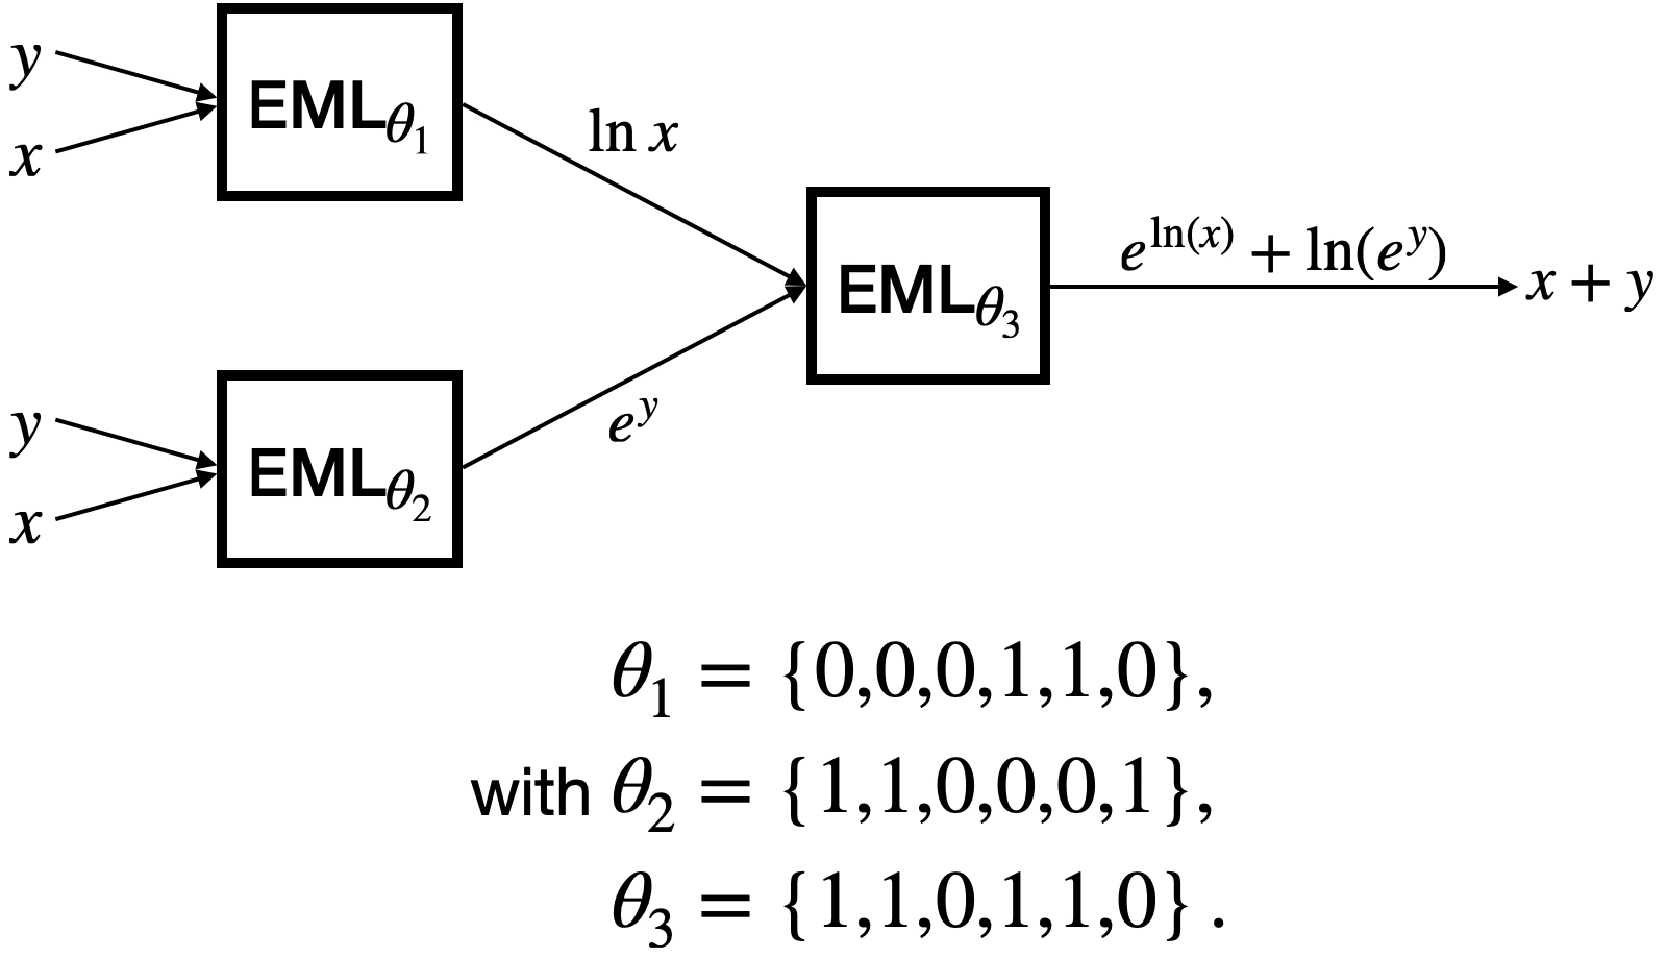
\includegraphics[width=\textwidth]{Figures/Addition.pdf}
    \caption{Addition (3)}
    \label{fig:addition}
  \end{subfigure}
  \hfill
  \begin{subfigure}{0.48\textwidth}
    \centering
    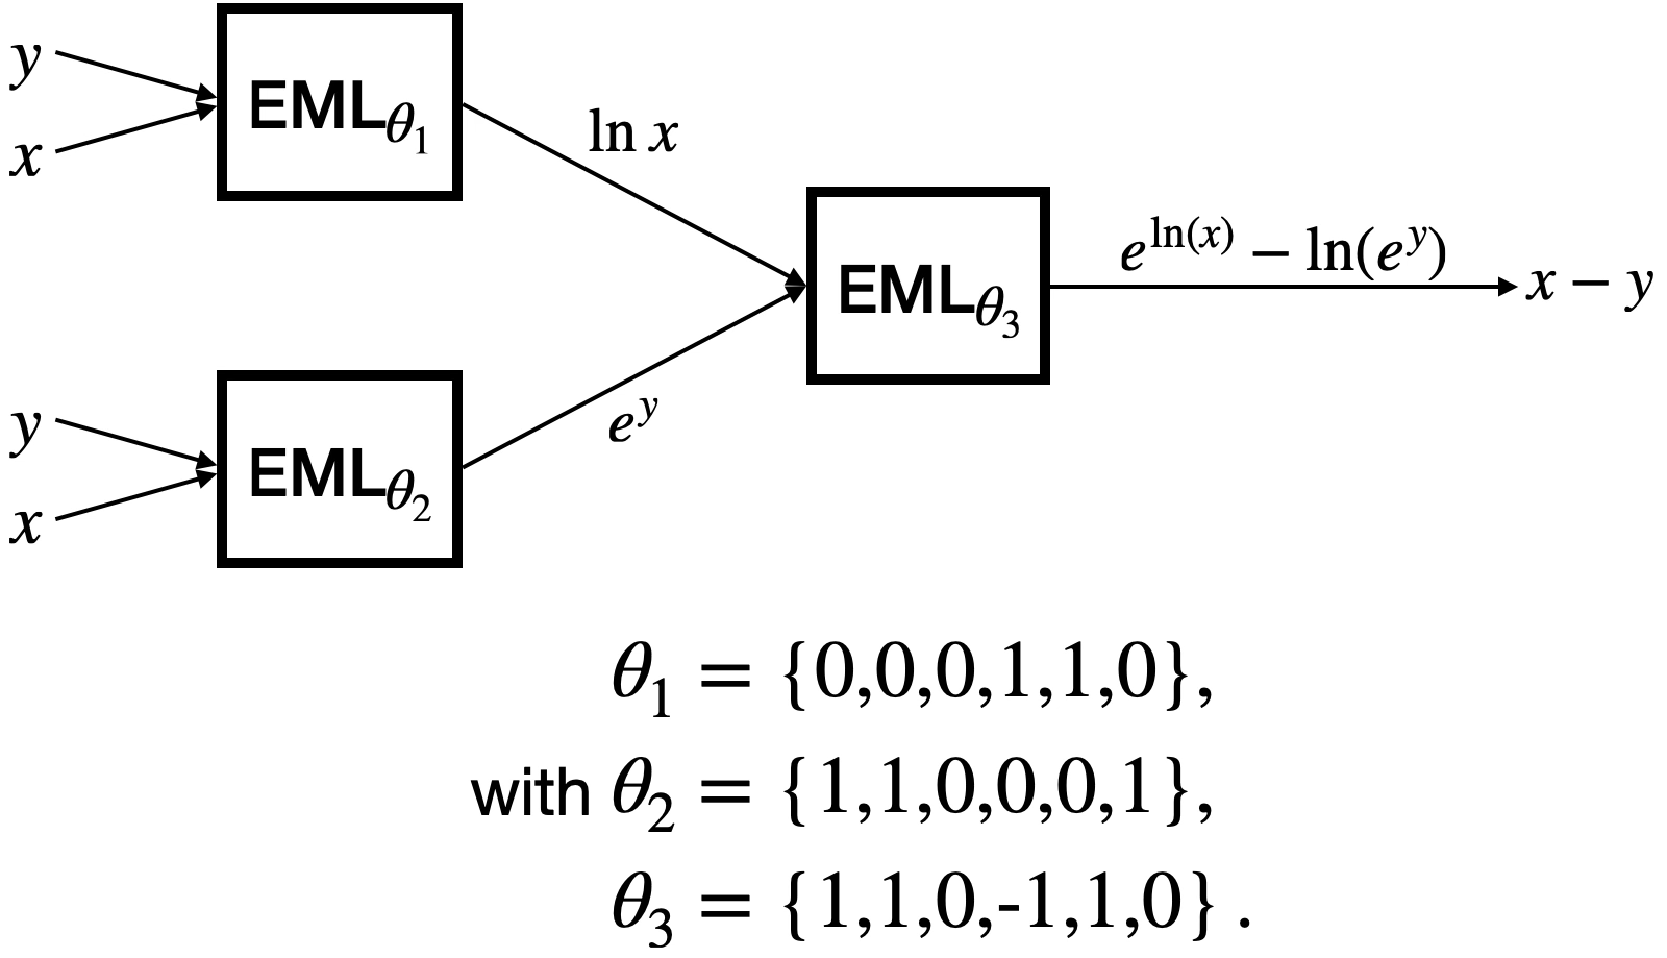
\includegraphics[width=\textwidth]{Figures/Subtraction.pdf}
    \caption{Subtraction (3)}
    \label{fig:subtraction}
  \end{subfigure}
  \vspace{1em}

  \begin{subfigure}{0.65\textwidth}
    \centering
    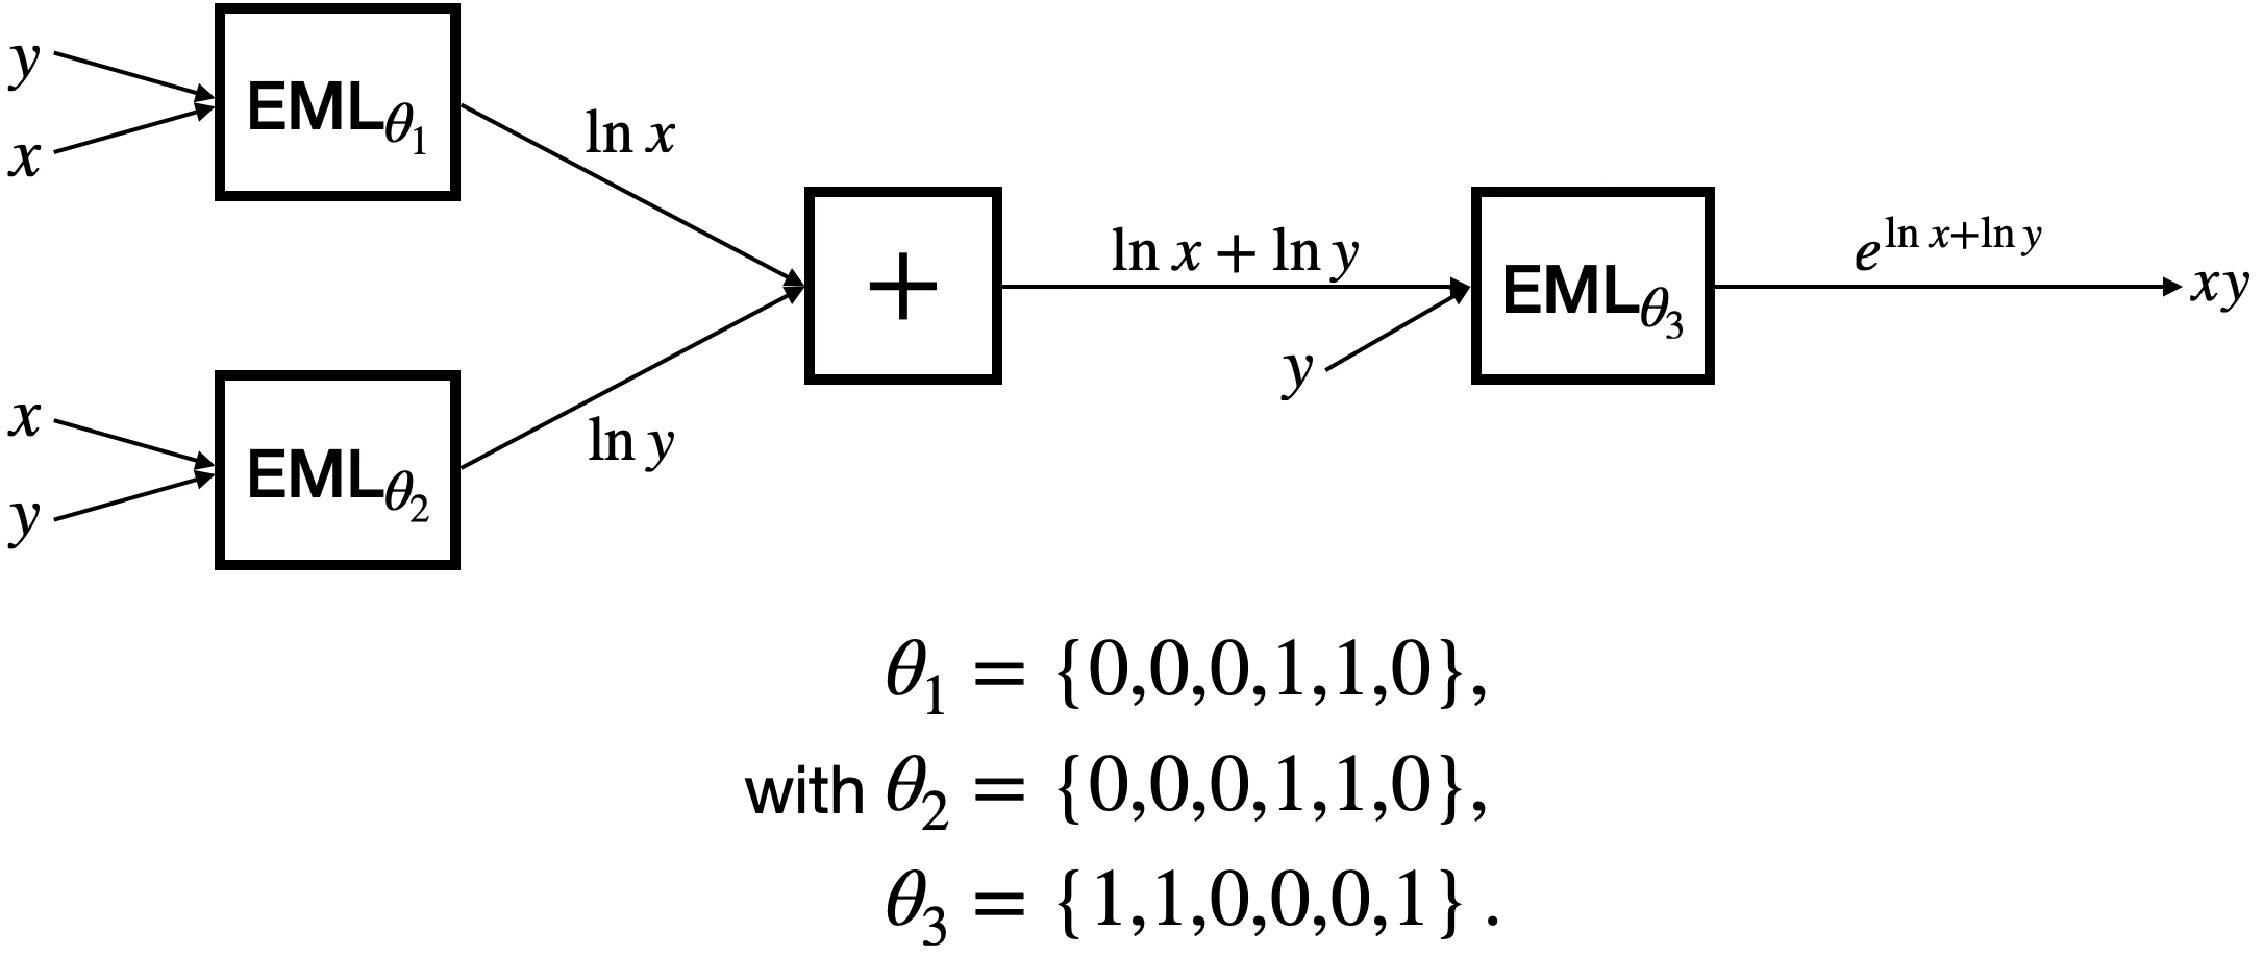
\includegraphics[width=\textwidth]{Figures/Multiplication.pdf}
    \caption{Multiplication (6)}
    \label{fig:multiplication}
  \end{subfigure}

  \vspace{1em}

  \begin{subfigure}{0.65\textwidth}
    \centering
    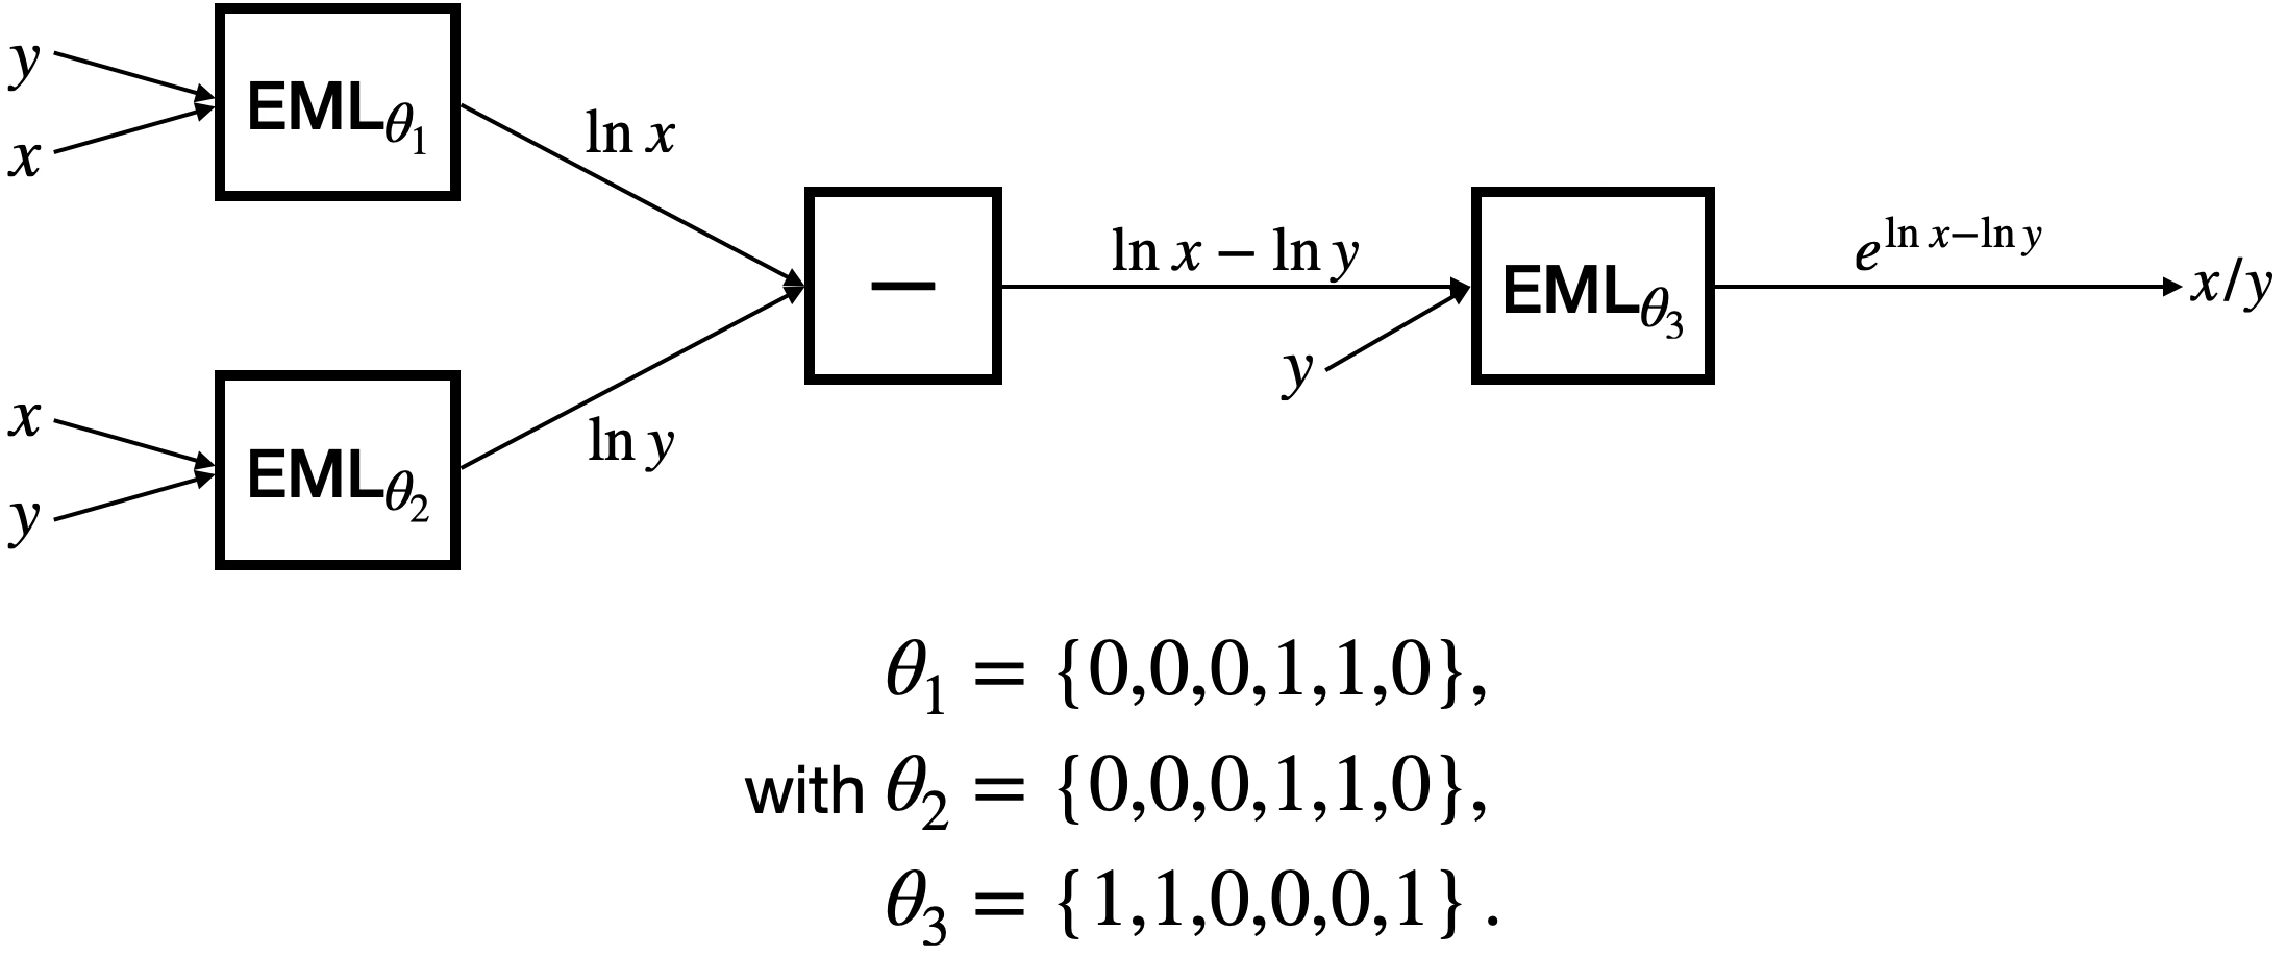
\includegraphics[width=\textwidth]{Figures/Division.pdf}
    \caption{Division (6)}
    \label{fig:division}
  \end{subfigure}
  
  \caption{The Basic Binary Operations}
  \label{fig:basicBinary}
\end{figure}

As observed in Figure \ref{fig:basicBinary}, we note that the size and depth requirements of these binary operations are summarized in Table \ref{tab:binary_ops}.
\begin{table}[h]
\centering
\begin{tabular}{c|cc}
Operator & $N(\cdot)$ & $\mathrm{Depth}(\cdot)$ \\
\hline
$x +_\theta y$ & 3 & 2 \\
$x -_\theta y$ & 3 & 2 \\
$x \times_\theta y$ & 6 & 4 \\
$x \div_\theta y$ & 6 & 4 \\
$x^n_\theta, \ m x^n_\theta$ & 2 & 2 \\
$\tanh_\theta (x), \ m\tanh_\theta(x)$ & 8 & 5
\end{tabular}
\caption{Size and depth of the operations in Appendix \ref{sec:basicBuildingBlocks}.}
\label{tab:binary_ops}
\end{table}
% \begin{itemize}
%     \item Addition: $N(+_\theta) = 3$ and $\text{Depth} (+_\theta) = 2$,
%     \item Subtraction: $N(-_\theta) = 3$ and $\text{Depth} (-_\theta) = 2$,
%     \item Multiplication: $N(\times_\theta) = 6$ and $\text{Depth} (\times_\theta) = 4$, and
%     \item Division: $N(\div_\theta) = 6$ and $\text{Depth} (\div_\theta) = 4$.
% \end{itemize}

\subsection{Exponentiation}
In our proof, we will also make frequent use of exponentiation to a constant power. We provide explicit constructions for EML trees that perform $x^n$ and $mx^n$ for constants $m,n \in \R$ in Figure \ref{fig:exponentiating}.
\begin{figure}[htbp]
  \centering
  \begin{subfigure}{0.6\textwidth}
    \centering
    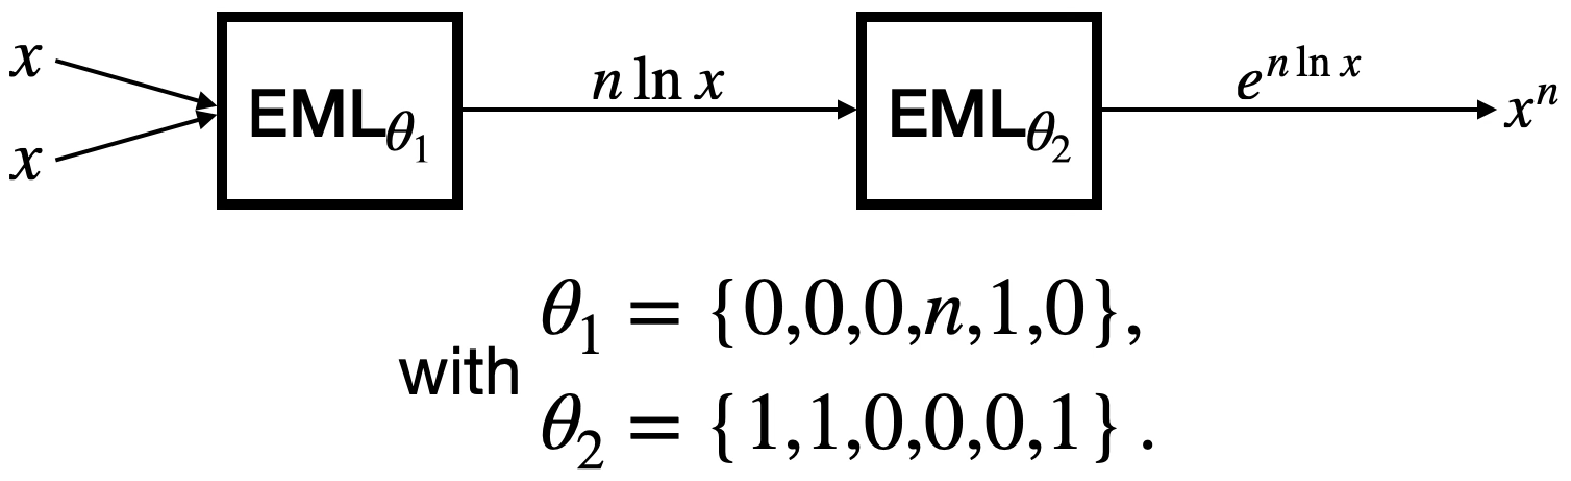
\includegraphics[width=\textwidth]{Figures/Exponentiation.pdf}
    \caption{Exponentiation to a constant $n$ (2)}
    \label{fig:exponentiationSec}
  \end{subfigure}
  \vspace{1em}
  \begin{subfigure}{0.6\textwidth}
    \centering
    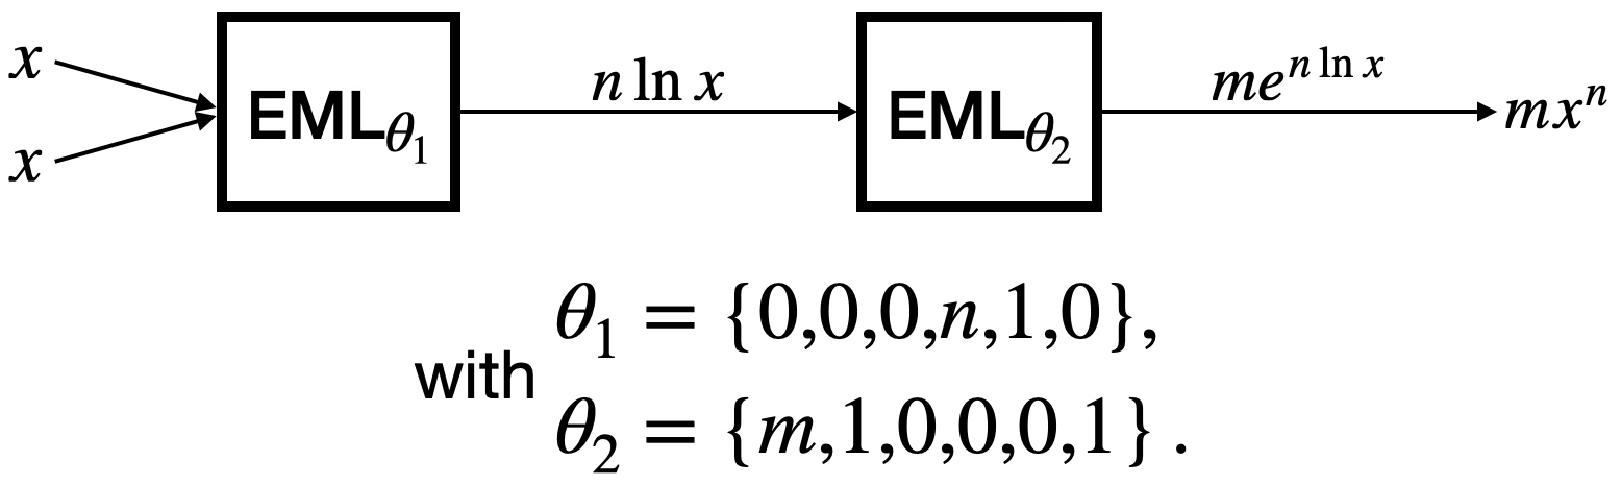
\includegraphics[width=\textwidth]{Figures/ExponentiationWithConstant.pdf}
    \caption{Exponentiation to a constant $n$ with prefactor $m$ (2)}
    \label{fig:exponentiationWithPrefactor}
  \end{subfigure}
  
  \caption{Exponentiating}
  \label{fig:exponentiating}
\end{figure}

Note that in Figure \ref{fig:exponentiationWithPrefactor}, we construct $m x^n$ directly, which we use to represent the monomial terms of polynomials (in Appendix \ref{sec:constructingPolynomials}). This is because it is more efficient to incorporate the coefficient within the exponentiation block itself, rather than introducing a separate multiplication block to combine a constant with the $x^n$ block.

For both exponentiation blocks (\ref{fig:exponentiationSec} and \ref{fig:exponentiationWithPrefactor}), the size and depth of the associated EML trees are $2$ (and appended to Table \ref{tab:binary_ops}).

% because to obtain the monomial terms of a polynomial, we have an associated coefficient, which is cheaper to obtain directly by changing the structure of the exponential block than to use a multiplication block to multiply a constant and the $x^n$ block. 

\subsection{Hyperbolic Tangent}
The hyperbolic tangent is constructed, using the exponential definition, by first getting $e^{2x} - 1$ and $e^{2x} + 1$ (via two separate EML blocks) and then diving them, as in Figure \ref{fig:tanhFigure}. The size of the $\tanh$ block is 8 and its depth is $5$, which are appended to Table \ref{tab:binary_ops}. 

We can similarly obtain $m \tanh x$, which is useful for the construction of the approximate partitions of unity, by amending the division block to include the prefactor $m$. This is done by changing $\theta_3$ in the division block (Figure \ref{fig:division}) to be $\theta_3 = \{m, 1, 0, 0, 0 , 1\}$.
\begin{figure}[htbp]
    \centering
    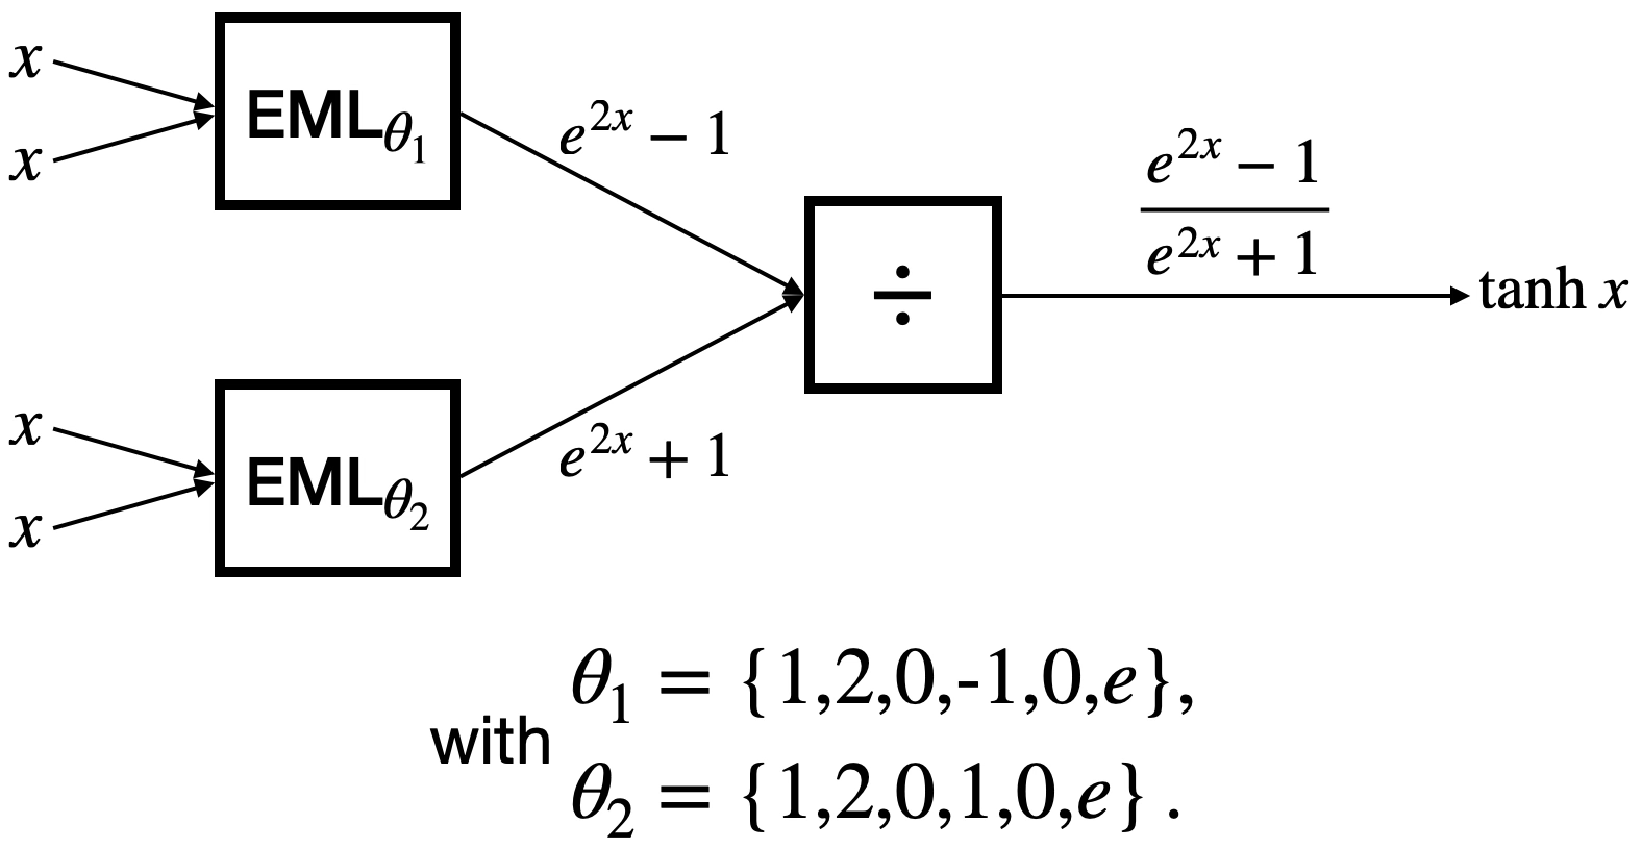
\includegraphics[width=0.6\linewidth]{Figures/HyperbolicTangent.pdf}
    \caption{Hyperbolic Tangent (8)}
    \label{fig:tanhFigure}
\end{figure}

\section{Constructing Polynomials}
\label{sec:constructingPolynomials}
The following two subsections detail how to construct univariate and multivariate polynomials using EML trees and provide upper bounds for the number of required EML blocks in each case.

\subsection{Univariate Polynomials}
A univariate polynomial of degree $k$, denoted by
\begin{equation}
    p(x) = \sum_{i=0}^k a_i x^i = a_0 + a_1 x + a_2 x^2 + \cdots + a_k x^k,
\end{equation}
can be (naively) constructed using EML blocks as in Figure \ref{fig:univariatePolynomial}, wherein we used two simple constituent blocks: addition (Figure \ref{fig:addition}) and exponentiation to a constant with a prefactor (Figure \ref{fig:exponentiationWithPrefactor}).

\begin{figure}[htbp]
    \centering
    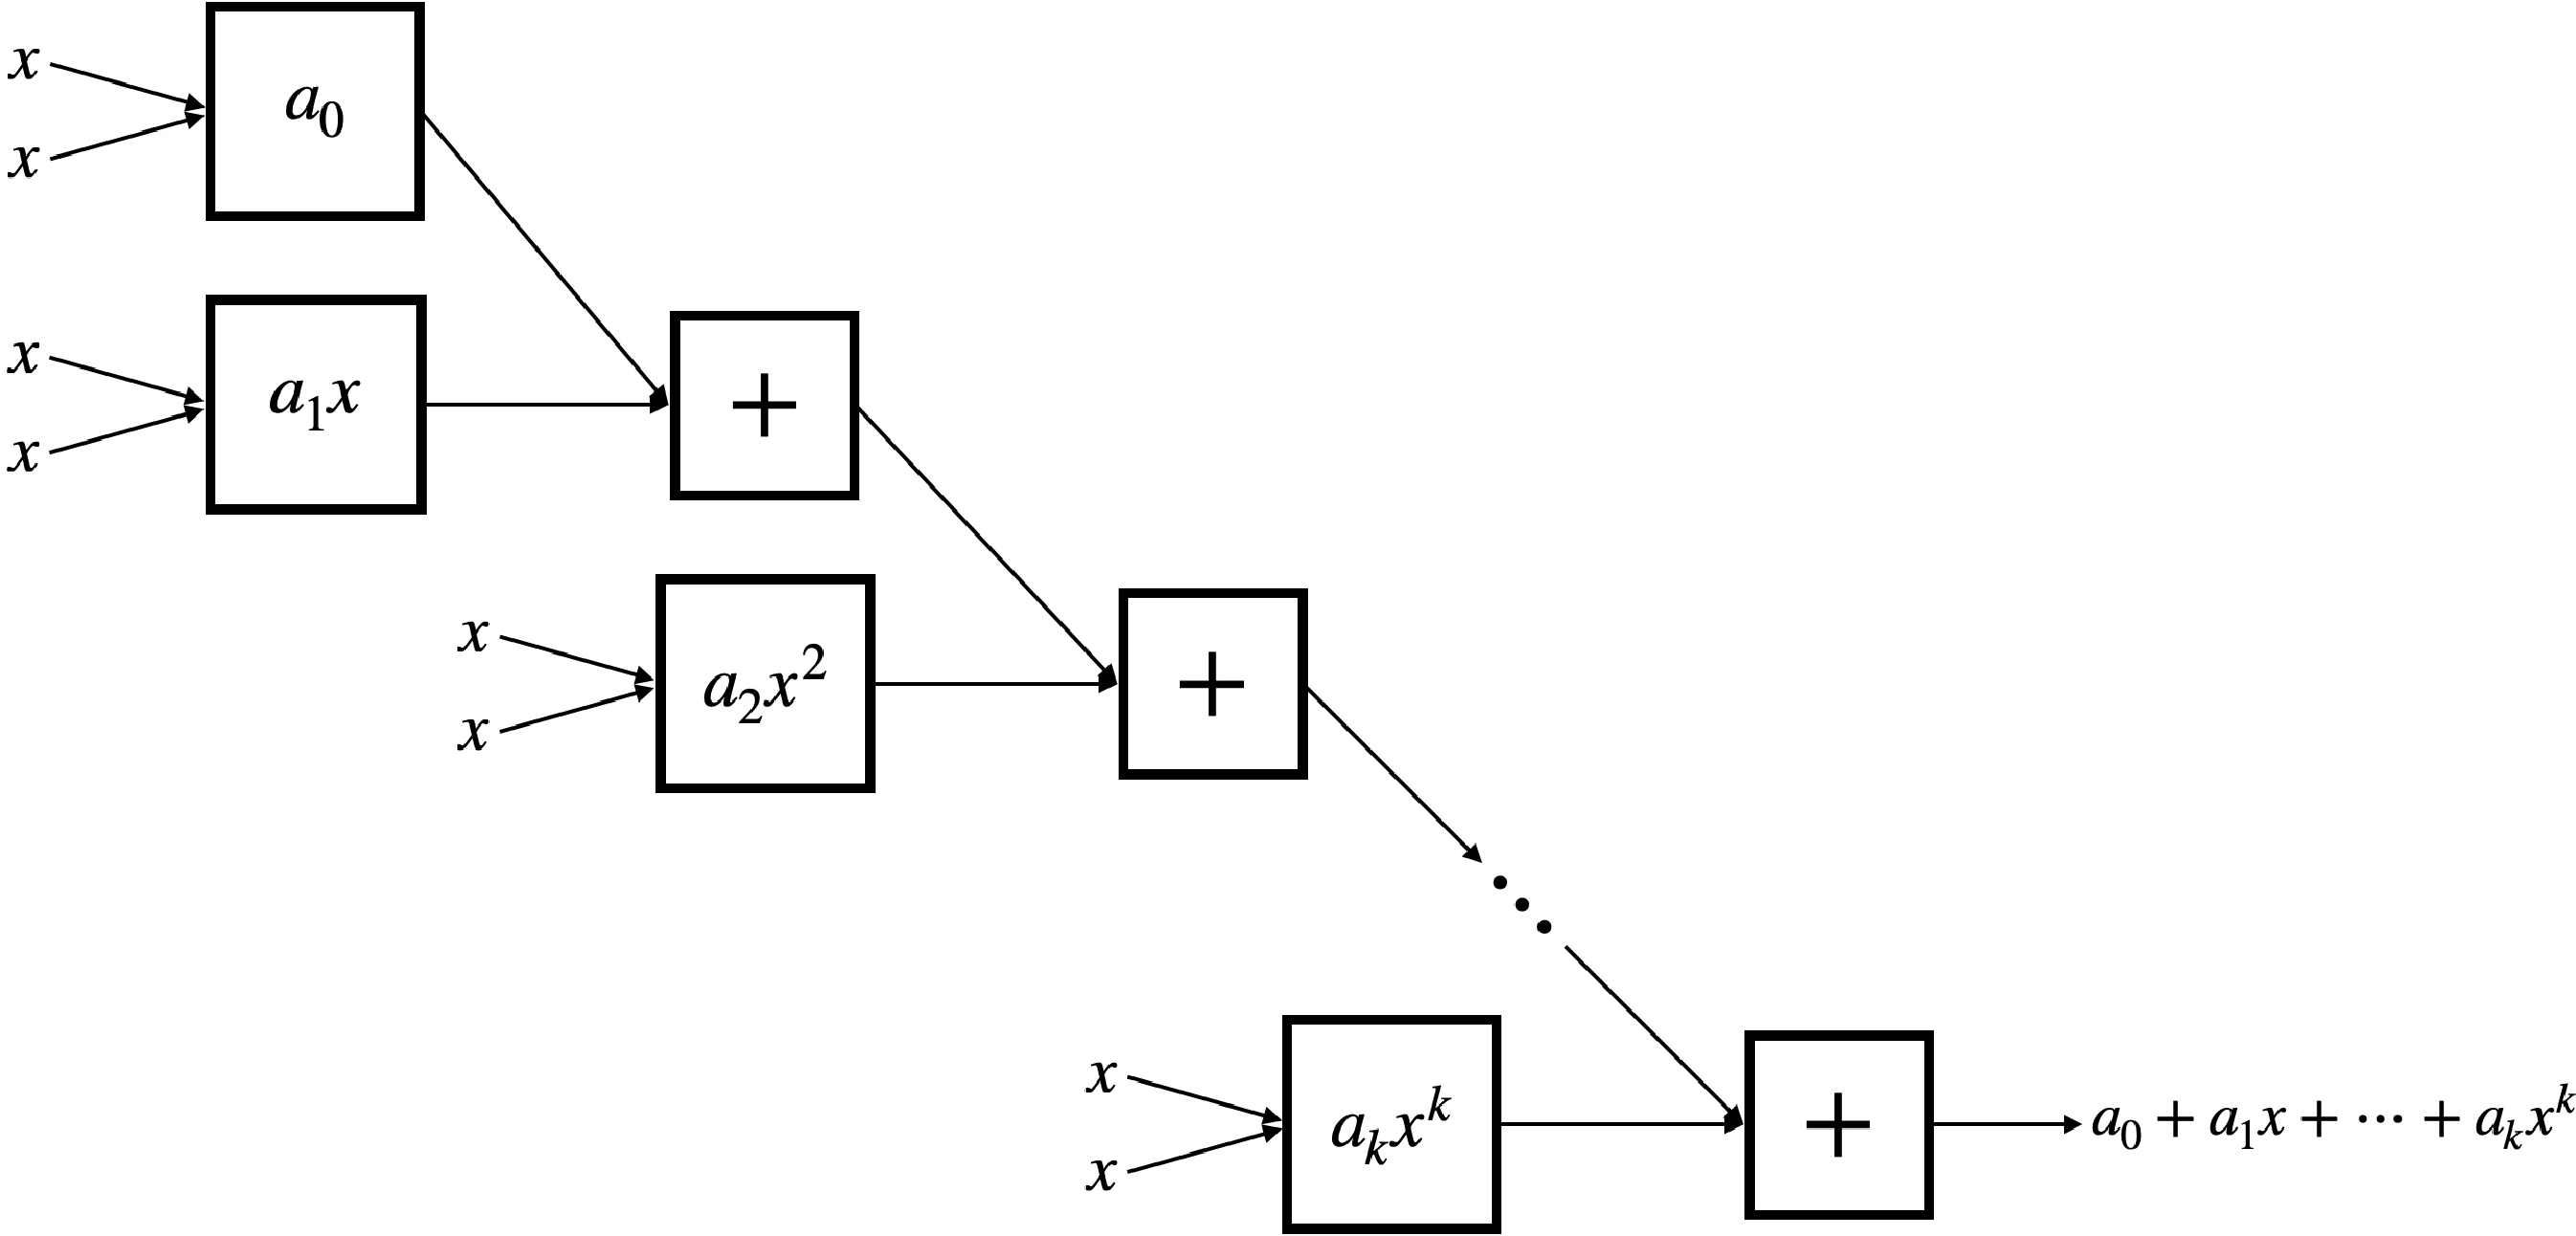
\includegraphics[width=0.9\linewidth]{Figures/Polynomial.pdf}
    \caption{Univariate Polynomial ($5s-3$)}
    \label{fig:univariatePolynomial}
\end{figure}

The upper bound on the number of required EML blocks is obtained by noting that we used
\begin{itemize}
    \item $k-1$ addition blocks (each requiring $3$ EML atoms), and
    \item $k$ exponentiation with a prefactor blocks (each requiring $2$ EML atoms).
\end{itemize}

So, constructing an EML tree $p_\theta$ such that $p_\theta = p$ (as per the above procedure) requires $N(T_\theta) = 3 (k - 1) + 2k = 5k-3$ and $\text{Depth} (T_\theta) = 2 + 2(k-1) = 2k$, since the longest path starts with the $x$ feeding into the $a_0$ block and passes through all $k-1$ addition blocks.

Hence, we phrase the above conclusion as the lemma:
\begin{lem}[Construction of Univariate Polynomials]
Given a univariate polynomial $p$ of degree $k$, there exists an EML tree $p_\theta$ (following the explicit construction in Figure \ref{fig:univariatePolynomial}), such that $p_\theta = p$ with $N(p_\theta) \leq 5k - 3$ and $\text{Depth}(p_\theta) \leq 2k$.
\end{lem}

\subsection{Multivariate Polynomials}
We recall that, for $\mathbf{x} = (x_1, \dots, x_d) \in \R^d$, a multivariate polynomial $p$ of degree $k$ is of the form
\begin{equation}
\label{multivariatePolynomial}
    p(\mathbf{x}) = \sum_{|\alpha| \leq k} c_\alpha x_1^{\alpha_1} x_2^{\alpha_2} \cdots x_d^{\alpha_d},
\end{equation}
where $\alpha = (\alpha_1, \alpha_2, \dots, \alpha_d)$ is a multi-index with $|\alpha| = \alpha_1 + \alpha_2 + \cdots + \alpha_d$, and $c_\alpha$ are the associated coefficients. Such a polynomial (of degree $\leq k$) has $\binom{d+k}{k}$ monomial terms.

To construct an EML tree for the polynomial \eqref{multivariatePolynomial}, (1) we construct the monomials $c_\alpha x_1^{\alpha_1}$, $x_2^{\alpha_2}$, $\dots$, $x_d^{\alpha_d}$ for each $\alpha$ with $|\alpha| \leq k$, (2) multiply these monomials together (separately for each $\alpha$), (3) do steps (1) and (2) for every monomial, and (4) add them together. A breakdown of the required EML tree sizes and depths for each step is as follows:
\begin{enumerate}[label=(\arabic*)]
    \item For a certain $\alpha$, each monomial, of which there are $d$, requires an exponentiation block (and the first has a prefactor), totaling $2d$ EML atoms;
    \item Again for each $\alpha$, we need to multiply the $d$ monomials, requiring $d-1$ multiplication blocks and, thus, $6(d-1)$ EML atoms; thus, each term, considering both getting monomials and multiplying them requires $2d + 6(d-1) = 8d - 6$ EML atoms; 
    \item Since we have $\binom{d+k}{d}$ terms in the polynomial, we do steps (1) and (2) $\binom{d+k}{d}$ times, thus requiring $(8d-6)\binom{d+k}{d}$ EML atoms;
    \item We finally sum over all terms, requiring $\binom{d+k}{d} - 1$ addition blocks, each consisting of $3$ EML atoms.
\end{enumerate}
Thus, in total, constructing the polynomial $p$ in \eqref{multivariatePolynomial} takes
\begin{equation}
    (8d-6) \binom{d+k}{d} + 3 \left( \binom{d+k}{d} - 1 \right) = (8d-3)\binom{d+k}{d} - 3
\end{equation}
EML atoms, and whose depth can be calculated (by drawing a schematic like Figure \ref{fig:univariatePolynomial}) to be
\begin{equation}
    2+4(d-1) + 2 \left( \binom{d+k}{d} - 1 \right) = 4d + 2 \binom{d+k}{d} -4,
\end{equation}
since the $x$'s feed into the first $c_\alpha x^{\alpha_1}$ block (of depth $2$), pass through $d-1$ multiplication (each of depth $4$), and then through $\binom{d+k}{d} - 1$ addition blocks (each of depth $2$).

The above justified the following lemma:
\begin{lem}[Construction of Multivariate Polynomials]
Given $p: \R^d \to \R$, a multivariate polynomial of degree $k$, there exists an EML tree $p_\theta$, such that $p_\theta = p$ with
\begin{equation}
    N(p_\theta) \leq (8d-3) \binom{d+k}{d} - 3, \quad \text{ and } \quad \text{Depth}(p_\theta) \leq 4d + 2 \binom{d+k}{d} - 4.
\end{equation}
\end{lem}

\section{Approximating the partition of unity}
In this section, we aim to construct an approximate partition of unity, similar to Section 4 of \cite{de2021approximation}. We do this because indicator functions are unsuitable to be represented by EML trees due to the fact that they contain a discontinuity and cannot be suitably represented by chaining elementary functions constructed from compositions of EML. 
For this reason, we construct smooth approximations of indicator functions on subsets of $[0,1]^d$ via $\tanh$ functions. When suitably shifted and parametrized, these functions output values close to $1$ within the subset and close to $0$ outside of it.

\subsection{Properties of the approximate partition of unity}
% To that effect, for every $j \in \mathcal{A}^N$, 
We first recall some of the properties of the partition of unity of \cite{de2021approximation}.

For a point $y \in \R$ and a parameter $\alpha \in \R$ (to be chosen later), we define the one-dimensional approximate indicator functions as
\be\begin{aligned}
\label{partitions_numero_uno}
    \rho_1^N(y) &= \fr{1}{2} - \fr{1}{2} \s \left( \alpha \left( y - \fr{1}{N} \right) \right), \\
    \rho_m^N(y) &= \fr{1}{2} \s \left( \alpha \left( y - \fr{m-1}{N} \right) \right)  - \fr{1}{2} \s \left( \alpha \left(y - \fr{m}{N} \right) \right) \quad \text{for } 2 \leq m \leq N-1, \\
    \rho_N^N(y) &= \fr{1}{2} \s \left( \alpha \left( y - \fr{N-1}{N} \right) \right) + \fr{1}{2}.
\end{aligned}\ee
We can clearly see that if $\alpha$ is large enough, these act as soft indicator functions over the intervals $\left(\fr{m-1}{N}, \fr{m}{N} \right)$ (depending on the subscript of $\rho$). 

To choose $\alpha$, we note that since $\s (x) \to 1$ as $x \to \infty$ and its derivatives also saturate ($\s^{(m)}(x) \to 0$ with $x \to \infty$), we can choose $R > 0$ large enough such that $|\s^{(m)}|$ is decreasing over $[R,\infty)$ for all $1 \leq m \leq k$.

So, given $\varepsilon > 0$, we choose $\alpha$, depending on $N$ and $\varepsilon$, large enough such that
\begin{equation}
    \fr{\alpha}{N} \geq R, \qquad 1 - \s \left( \fr{\alpha}{N} \right) \leq \varepsilon, \qquad \alpha^m \left| \s^{(m)} \left( \fr{\alpha}{N} \right) \right| \leq \varepsilon \text{ for all } 1 \leq m \leq k,
\end{equation}
justified also by Lemma A.4 in \cite{de2021approximation}. Consequently, $\alpha$ can be chosen to satisfy the above conditions and has the explicit value
\begin{equation}
\label{valueOfAlpha}
    \alpha = N \max \left\{ R, \ln \left( \fr{(2k)^{k+1} (Nk)^k}{e^k \varepsilon} \right) \right\},
\end{equation}
(see Lemma A.5 in \cite{de2021approximation} for justification).

% (In the paper \cite{de2021approximation}, they define a sequence of these functions for all $D \leq d$ since the proofs of the upcoming lemmas are done via an induction argument on dimension.)

Importantly, we define
\begin{equation}
\label{partition_of_unity_def}
    \Phi_j^{N} (x) = \prod_{i=1}^d \rho_{j_i}^{N} (x_i),
\end{equation}
which acts as our approximate partition of unity. We also define the set $\mathcal{V}_d$ as
\begin{equation}
    \mathcal{V}_d = \left\{ v \in \mathbb{Z}^d \ \middle| \ \max_{1 \leq i \leq d} |v_i| \leq 1 \right\},
\end{equation}
which allow us choose only the cubes directly surrounding a cube of interest.

Lemmas \ref{lemma1_partitionsOfUnity} and \ref{lemma2_partitionsOfUnity} below prove that the set of functions $\{ \Phi_j^N \}_{j \in \mathcal{A}^N}$ acts as an approximate partition of unity in the sense that they satisfy the following two properties: for every $j \in \mathcal{A}^N$,
\begin{equation}
    \sum_{v \in \mathcal{V}_d} \Phi_{j+v}^{N, d} \approx 1 \qquad \text{and} \qquad \sum_{\substack{v \notin \mathcal{V}_d, \\ j+v \in \mathcal{A}^N}} \Phi_{j+v}^{N,d} \approx 0.
\end{equation}

We recall the below two lemmas from \cite{de2021approximation}. The first provides a quantitative bound for how close to 1 is the contribution of $\Phi_j^N$ and its direct neighbors on $I_j^N$.
\begin{lem}[Lemma 4.1 of \cite{de2021approximation}]
\label{lemma1_partitionsOfUnity}
If $0 < \varepsilon < 1/4$, then
\begin{equation}
    \WnormD{\sum_{v \in \mathcal{V}_d} \Phi_{j+v}^{N} - 1}{k}{\infty}{I_j^N} \leq 2^{dk} d \varepsilon.
\end{equation}
\end{lem}

The second lemma guarantees that the contribution of the functions far away from the cube $I_j^N$ is small.
\begin{lem}[Lemma 4.2 of \cite{de2021approximation}]
\label{lemma2_partitionsOfUnity}
Let $k \in \N_0$ and $v \in \mathbb{Z}^d$ with $v_i \geq 2$ for all $1 \leq i \leq N$. Then, it holds that
\begin{equation}
\WnormD{\Phi_{j+v}^{N}}{k}{\infty}{I_j^N} \leq \max \{1, (2k)^{2k} \alpha^k \} \, \varepsilon.
\end{equation}
\end{lem}

\subsection{Constructing the approximate partition of unity using EML trees}
In Figure \ref{fig:partitionOfUnity}, we construct the $\rho_m^N$ functions for $2 \leq m \leq N-1$, according to the definition in \eqref{partitions_numero_uno}, and provide the associated parameters.
\begin{figure}[htbp]
    \centering
    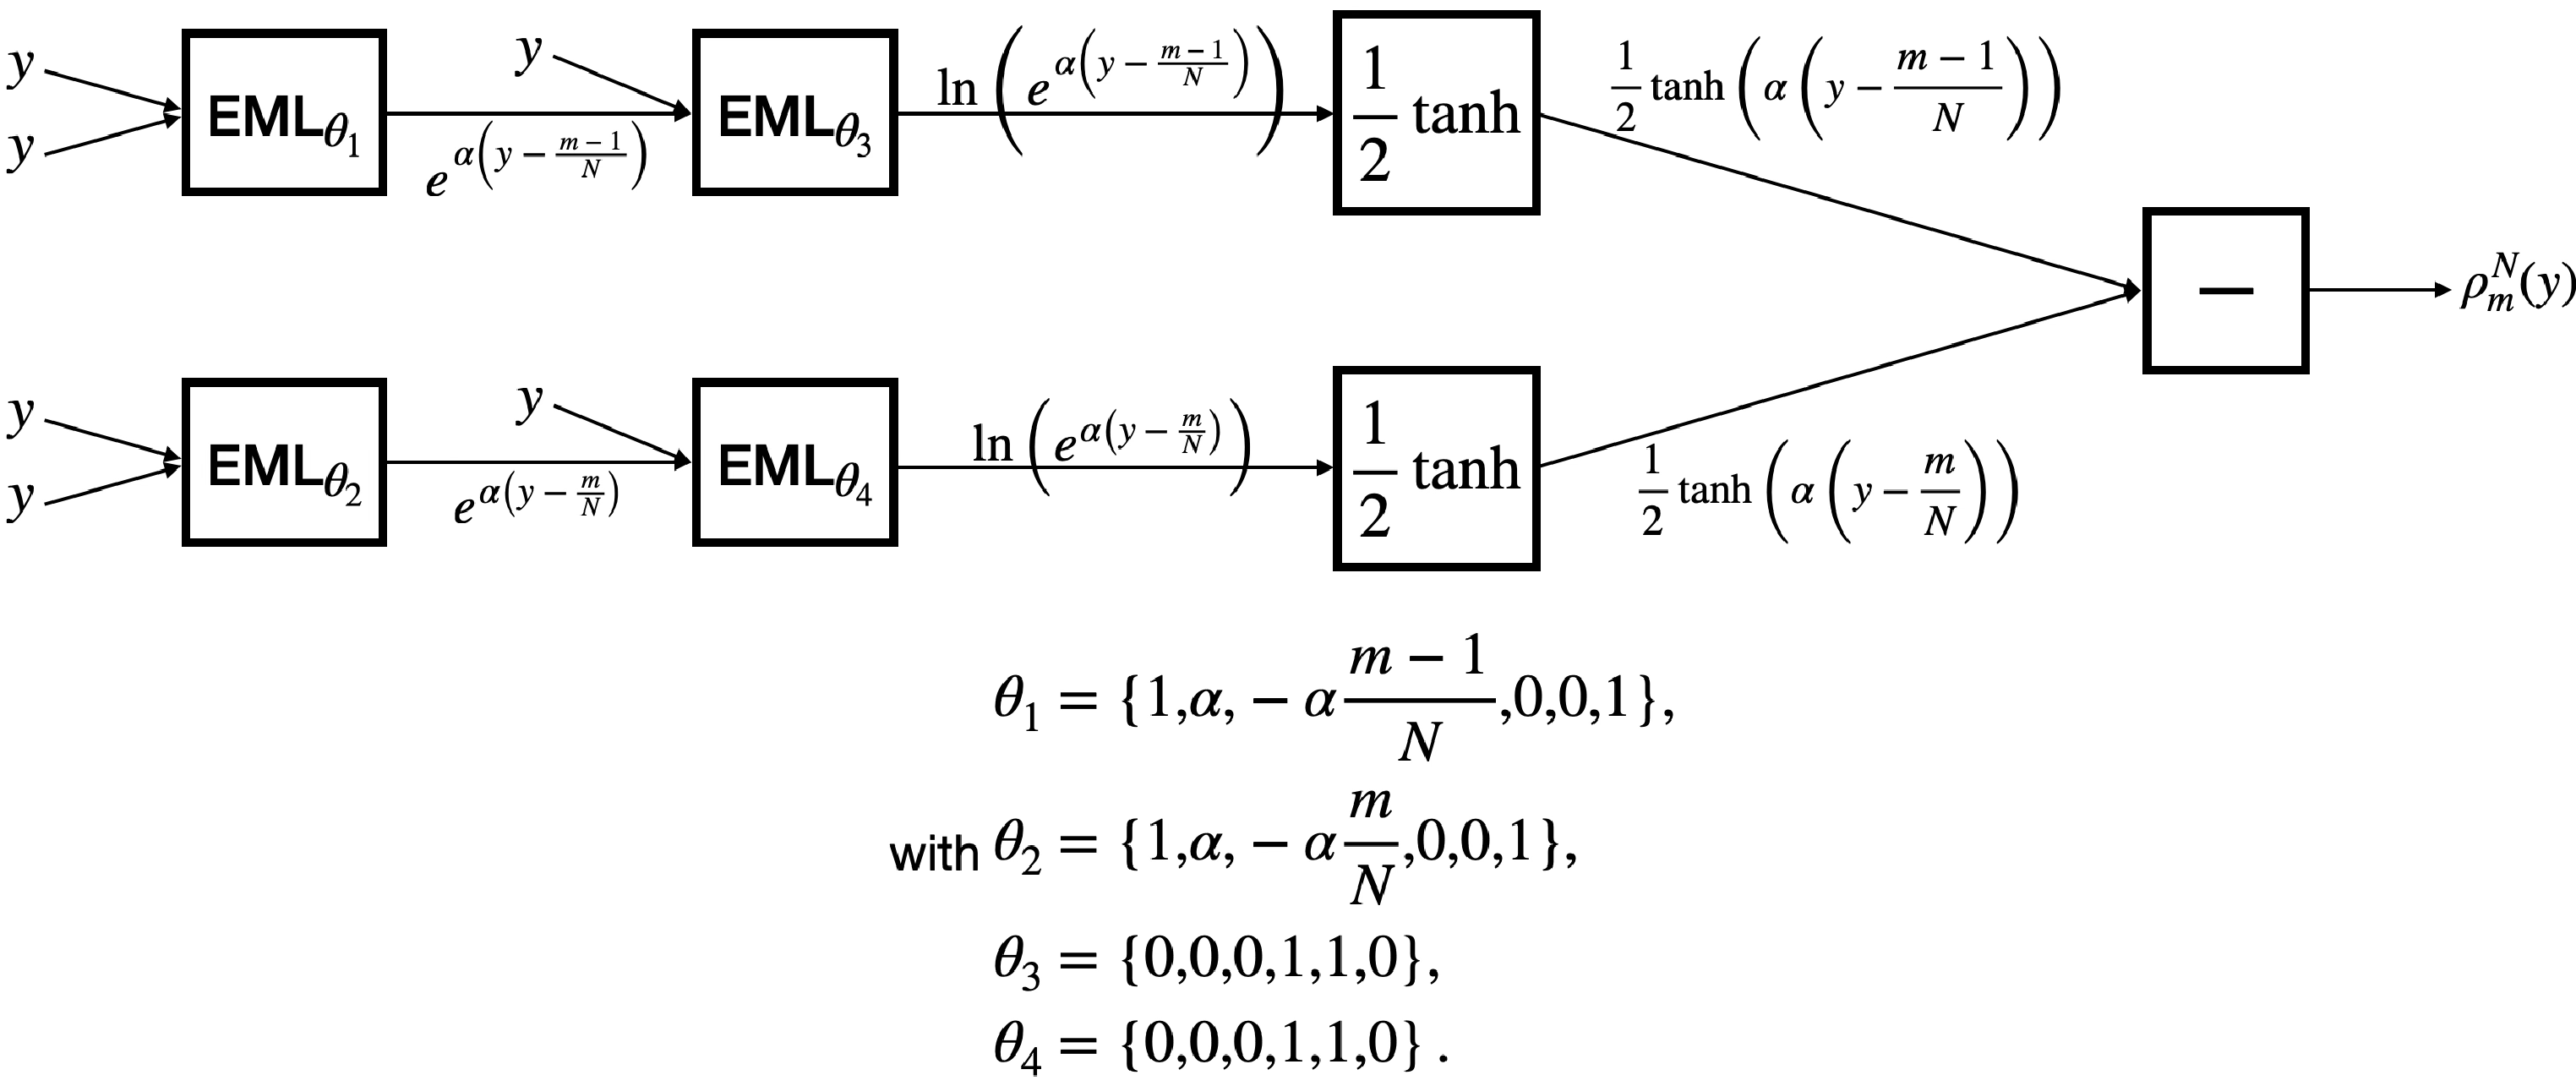
\includegraphics[width=0.99\linewidth]{Figures/PartitionOfUnity.pdf}
    \caption{Construction of $\rho_m^N$ for $2\leq m \leq N-1$}
    \label{fig:partitionOfUnity}
\end{figure}

This construction requires $4$ EML blocks, $2$ $\tanh$ blocks with $1/2$ constants, and a subtraction block, which boils down to a size of $4 + 2 \times 8 + 3 = 23$ and a depth of $1 + 1 + 5 + 2 = 9$.

$\rho_1^N$ and $\rho_N^N$ (from \eqref{partitions_numero_uno}) can be constructed more simply, requiring $3$ EML blocks (one of which to get the constant $1/2$), one $\tanh$ block, and one subtraction block, thus corresponding to a size of $3 + 8 + 3 = 14$ and depth of $1 + 1 + 5 + 2 = 9$. But, for the sake of simplicity, we will consider all instances of $\rho_m^N$ used to be those corresponding to Figure \ref{fig:partitionOfUnity}.

Then, we construct $\Phi_j^{N,d}$, using \eqref{partition_of_unity_def} by multiplying $d$ instances of the one-dimensional partitions, $\rho_{j_i}^N$. This requires $d-1$ multiplication blocks, and thus the EML tree corresponding to $\Phi_j^{N,d}$ has size $23 d + 6 (d-1) = 29d - 6$ and depth $9 + 4(d-1) = 4d + 5$, yielding the following lemma:
\begin{lem}[Construction of Approximate Partitions of Unity]
    For $N,d \in \N$ and $j \in \mathcal{A}^N$, there exists an EML tree $T_\theta$ such that $T_\theta = \Phi_j^{N}$ with
    \begin{equation}
        N(T_\theta) \leq 29d - 6, \quad \text{ and } \quad \text{Depth} (T_\theta) \leq 4d + 5.
    \end{equation}
\end{lem}

\section{Proof of Theorem \ref{main_theorem}}
\begin{proof}
We set out to perform the steps for the proof as described in the main text above and in Figure \ref{fig:sketchOfProof}.

{\bf{Step 1. Approximation by Local Polynomials.}}
We divide the domain $[0,1]^d$ into cubes of side length $1/N$. To denote these cubes, we use the corresponding index set
\begin{equation}
    \mathcal{A}^N = \{1, \dots, N\}^d % \{j \in \N^d \mid j_i \leq N \text{ for all } 1 \leq i \leq d \},
\end{equation}
of cardinality $|A^N| = N^d$. For every $j \in \mathcal{A}^N$, we associate the cube defined as 
\begin{equation}
    I_j^N = \bigtimes_{i=1}^d \left(\fr{j_i - 1}{N}, \fr{j_i}{N} \right).
\end{equation}
We also define overlapping cubes, which will be used to satisfy the condition for the Bramble-Hilbert lemma, for the given $N$ and every $j \in \mathcal{A}^N$ as
\begin{equation}
    J_j^N = \bigtimes_{i=1}^d \left(\fr{j_i - 2}{N}, \fr{j_i + 1}{N} \right),
\end{equation}
which is of diameter $\fr{3 \sqrt{d}}{N}$. We notice that there exists a ball of diameter $3/N$ such that $J_j^N$ is star-shaped with respect to every point in this ball (per Definition \ref{starShapedSet}). Thus, for every $j \in \mathcal{A}^N$, by the Bramble-Hilbert lemma (Lemma \ref{BrambleHilbert}), there exists a polynomial $p_j^N$ of degree at most $s-1$ such that, for all $0 \leq k \leq s-1$
\be\begin{aligned}
    \WnormD{f - p_j^N}{k}{\infty}{J_j^N} &\leq \fr{\pi^{1/4} \sqrt{s}}{(s-k-1)!} \left(\fr{5 d^2}{N} \right)^{s-k} \, |f|_{W^{s,\infty} ([0,1]^d)} \\
    &\leq \max_{0 \leq m \leq k} \fr{\pi^{1/4} \sqrt{s} (5d^2)^{s-m}}{(s-m-1)!} \fr{|f|_{W^{s, \infty} ([0,1]^d)}}{N^{s-k}} \coloneqq \fr{\mathcal{C} (d, k, s, f)}{N^{s-k}},
\end{aligned}\ee
choosing $N > 5d^2$ (to obtain decay) and using $3 \sqrt{e} \leq 5$.

\todo{\begin{rem}
    The polynomials are chosen to be good approximators on the overlapping cubes (not on the disjoint ones) because 
\end{rem}}

{\bf{Step 2. Definition of the Global Polynomial.}} We then define the global piecewise polynomial over the entire domain $[0,1]^d$ by
\begin{equation}
    p^N = \sum_{j \in \mathcal{A}^N} p_j^N \chi_j,
\end{equation}
where $\chi_j$ denotes the indicator function on $I_j^N$. Since $p^N$ is composed using indicator functions (which are discontinuous), it cannot be adequately controlled in $W^{k, \infty}$ spaces where $k \geq 1$. This is why we introduce
\begin{equation}
    \tilde{p}^N = \sum_{j \in \mathcal{A}^N} p_j^N \Phi_j^{N},
\end{equation}
as the global polynomial using the approximate partitions of unity and which we will ultimately represent using an EML tree. Similarly, we define $\tilde{f}^N$ as
\begin{equation}
    \tilde{f}^N = \sum_{j \in \mathcal{A}^N} f \, \Phi_j^{N}.
\end{equation}
% So
% \be\begin{aligned}
%     % \WnormO{f - p^N}{k}{\infty} = \WnormO{f - \sum_{j \in \mathcal{A}^N} p_j^N \chi_j}{k}{\infty} = \WnormO{\sum_{j \in \mathcal{A}^N} (f - p_j^N) \chi_j}{k}{\infty} 
% \end{aligned}\ee
% Hence, this achieves part $1$ of Figure \ref{fig:sketchOfProof}.

{\bf{Step 3. Approximation of $f$ by $\tilde{f}^N$.}} We first prove that $\tilde{f}^N$ is close to $f$. Considering an arbitrary $i \in \mathcal{A}^N$ and any $k \geq 1$, we employ the property \ref{banachAlgebraProperty}, Lemmas \ref{lemma1_partitionsOfUnity} and \ref{lemma2_partitionsOfUnity}, and the explicit value of $\alpha$ (from \eqref{valueOfAlpha}) to get
\be\begin{aligned}
    &\WnormD{f - \tilde{f}^N}{k}{\infty}{I_i^N} = \WnormD{f - \sum_{j \in \mathcal{A}^N} f \, \Phi_j^{N}}{k}{\infty}{I_i^N} \\
    &\quad \leq 2^k \WnormD{f}{k}{\infty}{I_i^N} \WnormD{1 - \sum_{v \in \mathcal{V}_d} \Phi_{i+v}^{N}}{k}{\infty}{I_i^N} + 2^k \WnormD{f}{k}{\infty}{I_i^N} \WnormD{\sum_{\substack{j \in \mathcal{A^N} \\ j-i \notin \mathcal{V}_d}} \Phi_j^{N}}{k}{\infty}{I_i^N} \\
    &\quad \leq 2^k \WnormD{f}{k}{\infty}{I_i^N} \left(2^{kd}d \varepsilon + N^d (2k)^{2k} \alpha^k \varepsilon \right) \\
    &\quad \leq 2^k \WnormD{f}{k}{\infty}{I_i^N} \left(2^{kd}d + N^d (2k)^{2k} N^k (k+1)^k \max \left\{R^k, \ln^k \left( \fr{2Nk^2}{\varepsilon^\fr{1}{k+1} e} \right) \right\} \right) \varepsilon \\
    &\quad \leq \delta (2(k+1))^{3k} \max \left\{R^k, \ln^k \left( \fr{2Nk^2}{\varepsilon^\fr{1}{k+1} e} \right) \right\} \fr{\mathcal{C}(d,k,s,f)}{N^{s-k}},
\end{aligned}\ee
with $\varepsilon$ chosen to satisfy
\begin{equation}
    \varepsilon \leq \fr{\delta \mathcal{C} (d,k,s,f)}{2^{(k+1) d} d N^{s+d} \, \WnormO{f}{k}{\infty}}.
\end{equation}
Similarly, for $k=0$, we have
\be\begin{aligned}
    \LnormD{f - \tilde{f}^N}{\infty}{I_i^N} \leq \LnormD{f}{\infty}{I_i^N} (d\varepsilon + N^d \varepsilon) \leq \fr{\delta}{3} \fr{\mathcal{C}(d,k,s,f)}{N^{s-k}}.
\end{aligned}\ee

{\bf{Step 4. Approximation of $\tilde{f}$ by the Global Polynomial $\tilde{p}^N$.}}
For $k = 0$,
\be\begin{aligned}
    &\LnormD{\tilde{f}^N - \tilde{p}^N}{\infty}{I_i^N} 
    = \LnormD{\sum_{j \in \mathcal{A}^N} (f - p_j^N) \, \Phi_j^N}{\infty}{I_i^N} \\
    &\qquad = \LnormD{\sum_{v \in \mathcal{V}_d} (f - p_{i + v}^N) \, \Phi_{i + v}^N}{\infty}{I_i^N} 
    + \sum_{\substack{j \in \mathcal{A}^N \\ j-i \notin \mathcal{V}_d}} \LnormD{f - p_j^N}{\infty}{I_i^N} \LnormD{\Phi_j^N}{\infty}{I_i^N} \\
    &\qquad \leq \left( \max_{v \in \mathcal{V}_d} \LnormD{f - p_{i+v}^N}{\infty}{I_i^N} \right) \LnormD{\sum_{v \in \mathcal{V}_d} \Phi_{i+v}^N}{\infty}{I_i^N} + \fr{\mathcal{C}(d,k,s,f)}{N^{s-k}} N^d \varepsilon \\
    &\qquad \leq \fr{\mathcal{C} (d,k,s,f)}{N^{s-k}}(1 + d\varepsilon) + \fr{\mathcal{C}(d,k,s,f)}{N^{s-k}}N^d \varepsilon \\
    &\qquad \leq \left( 1 + \fr{\delta}{3} \right) \fr{\mathcal{C} (d,k,s,f)}{N^{s-k}},
\end{aligned}\ee
with suitably chosen $\varepsilon$.

Whereas for $k\geq 1$,
\be\begin{aligned}
    &\WnormD{\tilde{f}^N - \tilde{p}^N}{k}{\infty}{I_i^N} 
    = \WnormD{\sum_{j \in \mathcal{A}^N} (f - p_j^N) \, \Phi_j^N}{k}{\infty}{I_i^N} \\
    &\qquad = \WnormD{\sum_{v \in \mathcal{V}_d} (f - p_{i + v}^N) \, \Phi_{i + v}^N}{k}{\infty}{I_i^N} 
    + \sum_{\substack{j \in \mathcal{A}^N \\ j-i \notin \mathcal{V}_d}} 2^k \LnormD{f - p_j^N}{\infty}{I_i^N} \WnormD{\Phi_j^N}{k}{\infty}{I_i^N} \\
    &\qquad \leq \text{\todo{something} } + N^d 2^k
\end{aligned}\ee

{\bf{Step 5. Finding the EML Tree.}}
In this step, our objective is to construct an EML tree $T^N$ such that it is exactly s exactly equal to the approximate global polynomial, that is $T^N = \tilde{p}^N$.

{\bf{Step 6. Conclusion.}}
Finally, 
\be\begin{aligned}
    &\WnormO{f - T^N}{k}{\infty} \\
        &\qquad \leq \WnormO{f - \tilde{f}^N}{k}{\infty} + \WnormO{\tilde{f}^N - \tilde{p}^N}{k}{\infty} + \WnormO{\tilde{p}^N - T^N}{k}{\infty} \\
        &\qquad \leq \WnormO{f - \tilde{f}^N}{k}{\infty} + \WnormO{\tilde{f}^N - \tilde{p}^N}{k}{\infty} \\
        &\qquad \leq 
\end{aligned}\ee

{\bf{Step 7. Upper Bound on the Size of the EML Tree.}}

% \begin{equation}
%     \tilde{p}^N = \sum_{j \in \{1, \dots, N\}^d} p_j^N \Phi_j^{N,d}
% \end{equation}

% \be\begin{aligned}
%     &\WnormO{f - T^N}{k}{\infty} \\
%     &\qquad \leq \WnormO{f - p^N}{k}{\infty} + \WnormO{p^N - \tilde{p}^N}{k}{\infty} + \WnormO{\tilde{p}^N - T^N}{k}{\infty}
% \end{aligned}\e

% {\bf{Step 2. .}}

\end{proof}

% \newpage

% \section{Introduction}
% The Exp-Minus-Log (EML) function attracted attention recently after the preprint \cite{eml} appeared. This is because the EML function is an continuous analogue of the NAND gate, that is all elementary functions can be expressed using it (and the digit $1$). The EML function is simply 
% \begin{equation}
%     \eml{x}{y} = \exp(x) - \ln (y).
% \end{equation}

% The set of elementary functions that it can single-handedly reconstruct are (i guess?):
% \begin{itemize}[leftmargin=*]
%     \item constants: $\pi, e, i, -1, 1, 2, x, y$,
%     \item functions: $\exp, \ln, \operatorname{inv}, \operatorname{half}, \operatorname{minus}, \operatorname{sqrt}, \operatorname{sqr}, \sigma, \sin, \cos, \tan, \arcsin, \arccos, \arctan, \sinh, \cosh, \\ \tanh, \operatorname{arsinh}, \operatorname{arcosh}, \operatorname{artanh}$,
%     \item operations: $+, -, \times, /, \log, \operatorname{pow}, \operatorname{avg}, \operatorname{hypot}$.
% \end{itemize}

% Put examples of combinations that give some of the above.

% Interetingly, does this look to you like a bit of EQL?

% The original paper talks about symbolic regression, interpretability, 

% Pros List:
% \begin{itemize}[leftmargin=*]
%     \item The proof we present is constructive.
%     \item We will have explicit growth rates / dependence of depth of tree on the desired epsilon.
%     \item EML is a very hot paper now, so why not ride the wagon?
% \end{itemize}

% Cons List:
% \begin{itemize}[leftmargin=*]
%     \item I am not sure how innovative the result is. I think it is pertinent and relevant to the discourse in the community (just based on the attention that the EML paper got), but I am not too familiar with the literature surrounding "tree" stuff to see if this is a good contribution.
%     \item The proof is not that hard once you realize that you can play with EML like Lego blocks. I was able to come up with the idea of the proof relatively fast.
%     \item There might be someone else who is trying to do the same thing, and dare I say might also attempt to submit to NeurIPS.
% \end{itemize}

% \section{The Proposed Network: $\text{EML}$}
% \todo{Find decent new names for all these things.}

% We also do it for (I guess to be more expressive for networks; it might make it shorter)
% \begin{equation}
%     \eml{x}{y} = \exp(ax+b) - \ln(cy + d).
% \end{equation}
% So,
% \begin{equation}
%     f = \eml{\eml{\dots}{\dots}}{\eml{\dots}{\dots}}
% \end{equation}

% \section{Proof of Universal Approximation}
% \todo{For the below proofs, give first a proof idea in words, and then do the math.}

% Do we directly do it for multidimensional input functions? It might be instructive to first prove it on 1D functions.

% \subsection{For Analytic Functions}
% Proof idea: We truncate up to a desired accuracy and we can actually construct the polynomial exactly using nested EML functions.

% We draw an explanatory figure showing that the global minimizer of the truncation of the analytic functions exists in the set.

% Include bound on size of set depending on order of truncation, which depends in turn on the desired accuracy of the approximation.

% \subsection{For Continuous Functions}
% Working on compact domain, we known that the set of analytic functions is dense in the set of continuous functions, so we can choose an analytic approximant desirably close to our wanted function, and then apply the result from the previous section.

% \section{Implementation}
% Maybe optimization might not be very easy because of the exponential function. Also, the logarithm only takes in positive values so that might cause some issues if not treated. we could apply absolute value or ReLU; I think the same result above will apply regardless.

% \section{Conclusion}
% It would be interesting if we could put our physics-informed hats on, and apply these things to equation discovery (KAN-style explorations of the benefit of their interpretability maybe). 

% Do the bounds get better if we work in different function classes (ex. barron spaces)?

% Can we say anything about spectral bias? Look at the ICLR 2025 paper: On the expressiveness and spectral bias of KANs

% Can we solve PDEs? Poisson, darcy flow? To prove these, we need approximation theory in sobolev spaces, which I think we could do, and then prove generalization and total error estimates.

% \begin{ack}
% Use unnumbered first level headings for the acknowledgments. All acknowledgments
% go at the end of the paper before the list of references. Moreover, you are required to declare
% funding (financial activities supporting the submitted work) and competing interests (related financial activities outside the submitted work).
% More information about this disclosure can be found at: \url{https://neurips.cc/Conferences/2026/PaperInformation/FundingDisclosure}.


% Do {\bf not} include this section in the anonymized submission, only in the final paper. You can use the \texttt{ack} environment provided in the style file to automatically hide this section in the anonymized submission.
% \end{ack}

% \section*{References}
\newpage
\bibliographystyle{plainnat}  % or abbrvnat, unsrtnat, …
\bibliography{bibliography.bib}

% References follow the acknowledgments in the camera-ready paper. Use unnumbered first-level heading for
% the references. Any choice of citation style is acceptable as long as you are
% consistent. It is permissible to reduce the font size to \verb+small+ (9 point)
% when listing the references.
% Note that the Reference section does not count towards the page limit.
% \medskip


% {
% \small


% [1] Alexander, J.A.\ \& Mozer, M.C.\ (1995) Template-based algorithms for
% connectionist rule extraction. In G.\ Tesauro, D.S.\ Touretzky and T.K.\ Leen
% (eds.), {\it Advances in Neural Information Processing Systems 7},
% pp.\ 609--616. Cambridge, MA: MIT Press.


% [2] Bower, J.M.\ \& Beeman, D.\ (1995) {\it The Book of GENESIS: Exploring
%   Realistic Neural Models with the GEneral NEural SImulation System.}  New York:
% TELOS/Springer--Verlag.


% [3] Hasselmo, M.E., Schnell, E.\ \& Barkai, E.\ (1995) Dynamics of learning and
% recall at excitatory recurrent synapses and cholinergic modulation in rat
% hippocampal region CA3. {\it Journal of Neuroscience} {\bf 15}(7):5249-5262.
% }


%%%%%%%%%%%%%%%%%%%%%%%%%%%%%%%%%%%%%%%%%%%%%%%%%%%%%%%%%%%%

% \appendix

%%%%%%%%%%%%%%%%%%%%%%%%%%%%%%%%%%%%%%%%%%%%%%%%%%%%%%%%%%%%

\newpage
\input{checklist.tex}

\end{document}